% Created 2013-07-26 Fri 18:59
\documentclass[a4paper,11pt]{article}
\usepackage[utf8]{inputenc}
\usepackage[T1]{fontenc}
\usepackage{fixltx2e}
\usepackage{graphicx}
\usepackage{longtable}
\usepackage{float}
\usepackage{wrapfig}
\usepackage{soul}
\usepackage{textcomp}
\usepackage{marvosym}
\usepackage{wasysym}
\usepackage{latexsym}
\usepackage{amssymb}
\usepackage{hyperref}
\tolerance=1000
\usepackage{fontspec}
\usepackage[titletoc,page,title]{appendix}
\usepackage{biblatex}
\usepackage{metalogo}
\usepackage{graphicx}
\usepackage{moreverb}
\usepackage{fancyvrb}
\usepackage{setspace}
\usepackage{subfig}
\usepackage[scientific-notation=true]{siunitx}
\usepackage{float}
\let\iint\relax % otherwise errors are thrown by amsmath. Defined in latexsym
\let\iiint\relax
\usepackage{amsmath}
\usepackage{hyperref}
\usepackage{tikz}
\usetikzlibrary{positioning}
\bibliography{fyp}
\defaultfontfeatures{Mapping=tex-text}
\setromanfont[Ligatures={Common},Numbers={Lining}]{Linux Libertine}
%% Change \maketitle to follow the SGS guidelines.
\renewcommand{\maketitle}
{\begin{titlepage}
\pagenumbering{roman}
%% Set the line spacing to 1 for the title page.
\begin{spacing}{1} 
\begin{large}
\begin{center}
\mbox{}
\vfill
\begin{sc}
Time Delay Estimation in Gravitationally Lensed\\ Photon Stream Pairs\\
\end{sc}
\vspace*{15mm}
Micha{\l} Staniaszek\\
Supervisor: Peter Ti{\v{n}}o\\
\vspace*{4mm}

\includegraphics[width=50mm,height=50mm]{images/crest.png}\\
For the degree of BSc Computer Science with Study Abroad\\
School of Computer Science\\
University of Birmingham\\
\vspace*{10mm}
\today
\vfill
\vspace*{.2in}
\end{center}
\end{large}
\end{spacing}
\end{titlepage}
}%\maketitle
\providecommand{\alert}[1]{\textbf{#1}}

\title{\noindent In this report, we present a system for estimating the time delay}
\author{\Large{Micha{\l} Staniaszek} \\\small{Supervisor: Peter Ti{\v{n}}o}}
\date{\today}
\hypersetup{
  pdfkeywords={},
  pdfsubject={},
  pdfcreator={Emacs Org-mode version 7.8.11}}

\begin{document}

\maketitle




\begin{abstract}
$\Delta$ between pairs of photon streams from separate images of gravitationally
lensed objects. Photon streams are simulated by generating arrival times of
individual photons using non-homogeneous Poisson processes with a rate function
$\lambda(t)$, which is randomly generated. We develop a linear estimator based
on ordinary least squares regression, and a kernel density estimator, which we
use to estimate the rate function of photon streams. Two time delay estimation
methods are developed, using inter-function area or probability density
functions to estimate the value of $\Delta$ based on estimates of the rate
function. We compare the efficacy of the four possible combinations of
estimation methods on sine functions and randomly generated functions, and show
that there is no significant difference between the accuracy of the estimates
they produce. However, the kernel density estimator combined with the
inter-function area method appears to be the most consistent.

\vspace{1.0cm}\noindent\textbf{Keywords:} Non-homogeneous Poisson process, gravitational lensing,
machine learning, linear regression, kernel density estimation
\end{abstract}

\vspace{2.0cm}\renewcommand{\abstractname}{Acknowledgements}
\begin{abstract} 
\noindent I would like to thank Peter Ti{\v{n}}o for his clear
 and insightful supervision, without which this project would not have been
 possible. Thanks also to Jeremy Wyatt, Nick Hawes and Achim Jung for their
 inspirational teaching and enthusiastic support during my time at university,
 and for sparking my interest in artificial intelligence and mathematics.
\end{abstract}

\begin{center}
\vspace*{\fill}\scriptsize{Typeset in Linux Libertine using \XeLaTeX}.
\end{center}

\newpage
\tableofcontents
\newpage
\pagenumbering{arabic}
\section{Introduction}
\label{sec-1}

  The continued advance of storage and sensing technology means that we are able
  to gather and store more data than ever. Gathering data is relatively simple
  in comparison to processing it, and with the volume of data available,
  choosing which data gets processed is becoming increasingly important. The
  Large Hadron Collider at CERN, for example, throws away tens of gigabytes of
  data each second, keeping only the most interesting data from the hundreds
  millions of collisions that occur \cite{WLCGproc}.

  The volume of data produced by modern telescopes, while not on the same scale
  as the LHC, is nonetheless overwhelming. Image sizes of one to two gigabytes
  are not uncommon, and deciding what data is actually relevant is not a trivial
  task \cite{starck2002handbook}. Using intelligent filtering algorithms, it
  should be possible to flag up interesting-looking data for further
  study. While there are many areas in which such capabilities would be useful,
  we are interested in creating the base of a system for finding potential
  gravitationally lensed objects---stars or galaxies whose light is bent because
  of high mass stellar objects in its path, creating multiple images of the
  object. To find such objects, we need to study the rate of arrival of photons
  from light sources in the sky, and try to find two or more of these photon
  \emph{streams} having the same characteristic function, which dictates how the
  arrival rate varies over time. Due to lensing effects, the streams from
  different images of the same object will have some time delay $\Delta$ between
  them. 
  
  Much work has been done in the astrophysics community to find more accurate
  estimates for the time delay of many lensed objects. An estimate of the
  possible range of time delays for the first observed lensed system, the quasar
  0967+561A, was given by Dyer and Roeder in 1980, a year after its discovery,
  with a value of between 0.03 and 1.7 years \cite{dyer1980range}. Since then,
  there have been many estimates of the time delay using various methods such as
  $\chi$$^2$ fitting and dispersion spectra, but the generally accepted value,
  determined by Kundi\'c et al. in 1997 is 417 $\pm$ 3 days
  \cite{kundic1997robust}. In this paper, a measurement of the global value of
  Hubble's constant is also made, indicating one useful application of the time
  delay. Increased accuracy of delay estimates increase the accuracy of the
  Hubble constant estimate. In addition, the time delay can be used to observe
  the distribution of dark matter in regions of space
  \cite{schneider2006gravitational}, and has also been proposed as a distance
  estimator \cite{bozza2004time}. For strongly lensed systems such as the above,
  time delays are generally large, and so daily flux measurements are sufficient
  to get a good idea of the characteristic function. In this project, we deal
  with time delays which are much shorter, on the order of minutes or hours, for
  which daily measurements do not provide enough data. For this reason, we
  consider the arrival times of individual photons.

  This report details the development of a system to estimate the time delay
  between two photon streams, which implements two methods of function
  estimation, and two methods of time delay estimation. The first function
  estimator extends a method introduced by Massey et
  al. \cite{massey1996estimating}, performing piecewise continuous function
  estimates. The second function estimator is a simplified implementation of the
  kernel density estimator presented by Cuevas-Tello et
  al. \cite{cuevas2006accurate}. We use two time delay estimation methods, one
  based on probability densities, and the other on the area between
  functions. We intend to perform a comparison of the efficacy of the various
  estimators implemented. One additional aim of the project is to create a
  system which might be useful in a larger system for automatically locating
  potential gravitationally lensed objects.

  In section \ref{sec-2} we discuss the concepts underpinning the project in more
  detail. In section \ref{sec-3} we introduce our method of
  generating random functions from Gaussians, and photon streams using Poisson
  processes. Section \ref{sec-4} shows our approach to estimating the
  underlying function of a given stream of photons. Our methods of calculating
  the time delays between multiple photon streams are explained in section
  \ref{sec-5}. Sections \ref{sec-6} and \ref{sec-7} give detailed
  information on the design and development of the system, including the
  software and project management aspects. Finally, in section \ref{sec-8}
  we present experimental data from both simulated and real data and discuss the
  relative effectiveness of our methods. We conclude in section \ref{sec-9} with
  a summary of the achievements of the project, suggestions for further work and
  potential improvements, and some individual comments.
\section{Background}
\label{sec-2}
\subsection{Gravitational Lensing}
\label{sec-2-1}

   In an eight-year period starting in 1907 and ending in 1915 with the
   publication of a paper on the field equations of gravitation
   \cite{einstein1915general}, Albert Einstein wrote many papers developing a
   new theory of gravitation, his general theory of relativity. This
   generalisation of special relativity and Newton's law of universal
   gravitation led to a revolution in physics, and remains one of the most
   important scientific advances to date. The theory describes how spacetime is
   affected by the presence of matter. The idea has many important consequences,
   but one is of particular relevance in the context of this report.

   According to the theory, objects with mass, or \emph{massive} objects, cause
   spacetime, a mathematical model which combines space and time into a single
   ``object'', to curve around them. A simple way to visualise this effect is to
   imagine dropping a ball onto a sheet of cloth which has been pulled taut. The
   ball will eventually come to a stop in the centre of the cloth, and cause it
   to sag. The sheet represents spacetime, and the ball represents anything from
   planets, to stars, or even entire galaxies. Depending on the weight of the
   ball, the shape of the cloth will be affected to different degrees---a ping
   pong ball will have hardly any effect at all, but if we drop a bowling ball
   onto the sheet, the effect will be very apparent. In a similar way, the
   amount that spacetime curves around an object depends on its mass. Objects
   with high mass curve the sheet a lot, and objects with low mass only a
   little. If a second ball, lighter than the first, is introduced to the
   system, what happens?  With no initial velocity, it will roll in a straight
   line towards the first ball sitting at the centre of the sheet. This is one
   way of thinking about gravity and its relationship with spacetime---an
   object's gravitational attraction is a result of its mass curving spacetime,
   and the strength of the attraction is proportional to the mass. While objects
   with no mass, such as photons, cannot be affected by gravity directly, they
   \emph{are} affected by the curvature of spacetime. This bending of light rays
   is known as \emph{gravitational lensing}. In our example, lensing can be
   imagined as the change in the trajectory of a ball which is pushed at an
   angle towards a ball sitting in the centre of the cloth.
   \begin{figure}[h]
   \centering
   \subfloat[An Einstein ring]{
   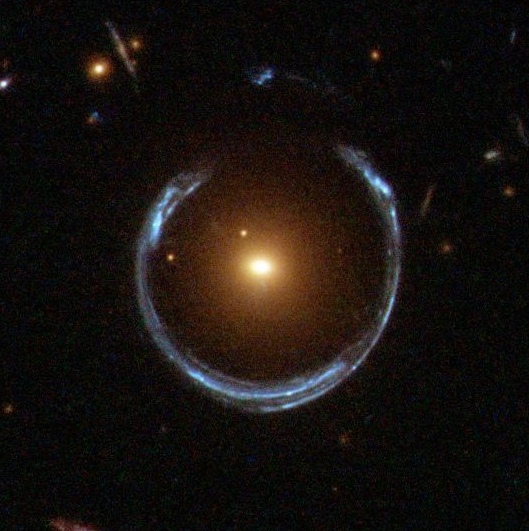
\includegraphics[width=0.4\textwidth]{images/einstein_ring}
   \label{fig:einring}
   }
   \qquad
   \subfloat[Einstein's cross]{
   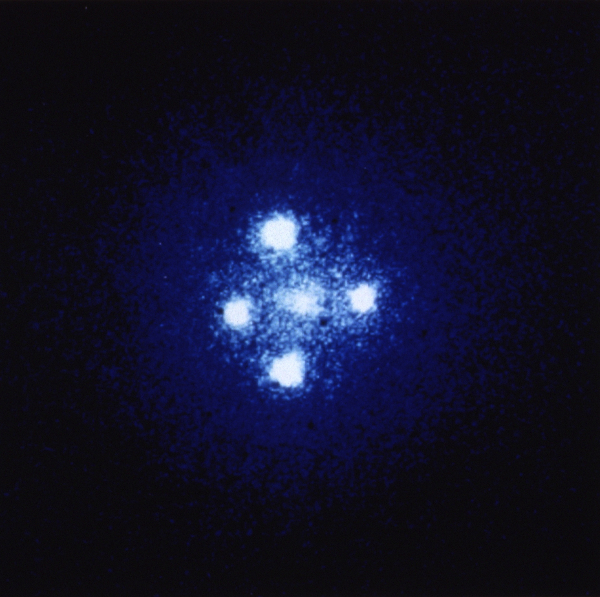
\includegraphics[width=0.4\textwidth]{images/einstein_cross}
   \label{fig:einsteincross}
   }
   \caption{Two examples of strong lensing effects. a) shows light from
   a distant blue galaxy being distorted by the central galaxy LRG 3-757
   \cite{einsteinring}. b) shows four images of a distant quasar being lensed by a
   foreground galaxy \cite{eincross}.}
   \label{fig:stronglens}
   \end{figure}
   The first person to study the effects of gravitational lensing was Orest
   Chvolson, publishing a short note to \emph{Astronomische Nachrichten} in 1924
   \cite{chwolsonlensing}. However, the concept was largely unknown until a
   short calculation by Einstein was published in \emph{Science} in 1936
   \cite{einsteinlensing}. Interestingly, Chvolson's note appears directly above
   a note from Einstein\cite{einsteinchwolson}, but there appears to be no
   evidence that Einstein had ever seen it \cite{renn2000eclipses}. The first
   gravitationally lensed object to be identified was the twin quasar SBS
   0957+561, in 1979, and since then, over a hundred such objects have been
   discovered \cite{firstlens,gravlenscount}. The effect of gravitational
   lensing is, as the name suggests, similar to that of a lens, such as that of
   a camera. Unlike a camera lens, however, gravitational lenses do not have a
   focal point, but instead a focal line, resulting in images such as that shown
   in Figure \ref{fig:einring} if the source (the object being lensed), the
   lensing object (the massive object around which the light is being bent) and
   the observer lie on a straight line. This effect is relatively rare, however,
   and in general rather than a ring, multiple images of the source can be
   observed. In these so called \emph{strong} lensing effects, the distortion is
   very clearly visible. However, two other classes of lensing
   exist---\emph{weak lensing} and \emph{microlensing}.  The effects of weak
   lensing cannot easily be observed visually, but statistical techniques can
   show the distortion produced. Microlensing works on even smaller scales than
   the other two classes, and can be used to detect planets and stars. It has
   also been proposed as a method to find objects such as black holes and brown
   dwarfs, which are otherwise difficult to detect
   \cite{schneider2006gravitational}.
\subsection{Poisson Processes}
\label{sec-2-2}

   There are many situations in which one can benefit from a good model of the
   number of events of interest that occur in a given period. Poisson processes
   are \emph{stochastic processes} that can be used to create such models. A
   stochastic process is a collection of random variables that represents the
   evolution of a system over time. Such processes do not evolve in a
   \emph{deterministic} way. That is, the way they change as time passes is not
   predictable. Poisson processes are part of a family of stochastic processes
   which count the number of events and their time of occurrence in a given
   interval. They have been used to model the number of incoming requests to a
   server \cite{arlitt1997internet}, as well as many other time-related
   systems. In their basic form, Poisson processes have the following important
   properties \cite{ross1997simulation}:
\begin{enumerate}
\item $N(0)=0$.
\begin{itemize}
\item $N(t)$ represents the total number of events that occurred up until time
     $t$. Thus, if $N(0)=0$, it follows that the process begins at $t=0$.
\end{itemize}
\item The numbers of events occurring in disjoint time intervals are independent.
\begin{itemize}
\item The \emph{independent increment} assumption. This states that $N(t)$, the
     number of events that occur up to time $t$ is \emph{independent} of the
     number $N(t+s)-N(t)$, i.e. the number of events in the time interval
     between $t$ and $s$. In other words, the number of events that occur in one
     interval does not have any effect on the number of events in any other time
     interval with which it does not overlap.
\end{itemize}
\item The probability distribution of the number of events that occur in a given
   interval is dependent only on the length of the interval.
\begin{itemize}
\item The \emph{stationary increment} assumption. The implication of this is that
     the probability distribution of $N(t+s)-N(t)$ is the same for all values of
     $t$. That is, the likelihood of $n$ events occurring in the above time
     interval does not change, regardless of the value of $t$.
\end{itemize}
\item No counted occurrences are simultaneous.
\begin{itemize}
\item For all events that occur in the duration of the process, no two events
     will occur at the same time.
\end{itemize}
\end{enumerate}

   Each Poisson processes is governed by a \emph{rate parameter}, $\lambda$,
   which represents the number of events that occur in each time interval, on
   average. As we are counting events, it is clear that the rate parameter can
   never go below zero---there cannot be a negative number of events in a given
   time interval. There are two types of Poisson processes, \emph{homogeneous}
   and \emph{non-homogeneous}. In a homogeneous Poisson process (HPP), the rate
   parameter is constant for the entirety of the process. This means that in
   every interval, the same number of events are likely to occur. In contrast, a
   non-homogeneous Poisson process (NHPP) has a rate parameter which
   varies. This means that the rate at which events occur varies as the process
   evolves. As such, the value of $\lambda$ becomes a function of time, written
   as $\lambda(t)$, called the \emph{rate function}. As a result, the stationary
   increment assumption does not apply to NHPPs. Figure \ref{fig:poisson} shows
   some examples of how the Poisson process evolves over time.
   \begin{figure}
   \subfloat[Homogeneous]{
   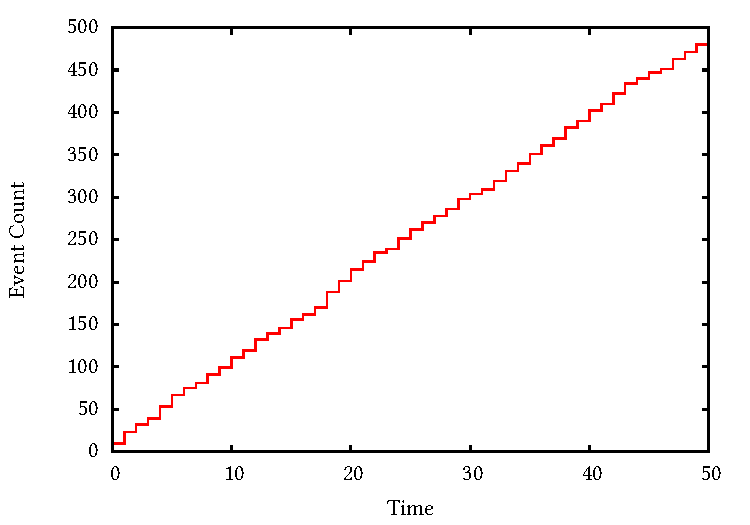
\includegraphics[width=0.5\textwidth]{images/homplot}
   }
   \subfloat[Non-homogeneous]{
   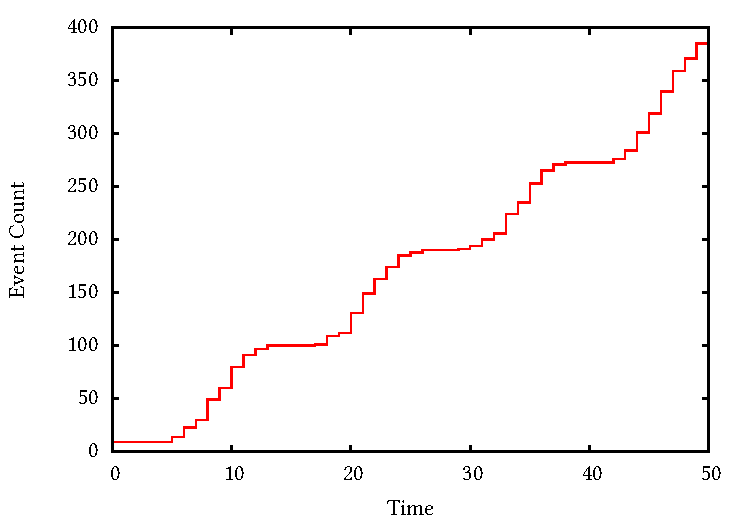
\includegraphics[width=0.5\textwidth]{images/nonhomplot}
   }
   \caption{Two examples of Poisson process paths. The homogeneous process has a
   rate parameter $\lambda=$ 10, and the non-homogeneous rate parameter varies
   depending on the value of a sine function.}
   \label{fig:poisson}
   \end{figure}
\subsection{Regression}
\label{sec-2-3}

   Regression is a statistical technique used to fit lines or curves to data
   points in order to find some sort of relationship between them. The number of
   variables in the data is important. One of the variables is called a
   \emph{dependent} variable. We want to find the relationship between this
   variable and the other variables, called \emph{independent}
   variables. Consider the expression $y=f(x)$. If $f(x)$ is some function of
   the variable $x$, then we know that the value of $y$ depends on the value of
   $x$, and so $y$ is the dependent variable, and $x$ is the independent
   variable. In linear regression, there can be multiple independent variables,
   but only a single dependent variable. In order to fit a line to data, a
   \emph{predictor function} is used. This function predicts the value of the
   dependent variable, as we can never know its true value as we are only able
   to use a statistical sample of data from the random variable. Regression is
   used in fields ranging from epidemiology to economics. An example of its use
   is finding factors contributing to smoking initiation and cessation
   \cite{van2005determinants}.
\section{Simulation of Photon Streams}
\label{sec-3}

  The first step in building the system was the development of a photon stream
  simulator. The ability to simulate photon streams means that the system can be
  tested on many different stream types, so that we are able to determine where
  its strengths and weaknesses lie. While many simulation tools are very
  complex, our system does not require simulation of the source objects or the
  movement of photons, as we are only interested in their arrival time. A source
  can be represented by a random variable which indicates its variability with
  time. Different types of sources will have different types of characteristic
  functions---the variation in a quasar will be very different to that of an
  individual star, for example. A NHPP is an ideal way to model this type of
  system. The function $\lambda(t)$ is the rate function of the process, and the
  times output by the process will represent the arrival times of the
  photons. $\lambda(t)$ provides a rate parameter at each time $t$ for the
  duration of the simulation.
\subsection{Function Generation}
\label{sec-3-1}

   To generate random functions, we make use of Gaussians. The generation process
   involves four simple steps:
\begin{enumerate}
\item Pick some value $\Delta t$ which represents the distance between the mean
   $\mu$ of successive Gaussians.
\item Define some value $\alpha$, where the standard deviation $\sigma$ of each
   Gaussian is determined by $\alpha\cdot\Delta t$.
\item For each Gaussian, choose some weight $w_i$, from a uniform distribution
   between -1 and 1, and scale it by some multiplier.
\item Using some step $s$, sum all the Gaussians at each point on the $x$-axis which
   we get from these $s$ values.
\end{enumerate}

   The first step defines how spread out the Gaussians should be in the interval
   $[t_0, T]$ in which the function is to be generated. If the spread is large,
   then depending on the standard deviation of the Gaussians there will be many
   points in the interval where the value of the rate function is zero. On the
   other hand, with a low value of $\Delta t$, most points on the line should
   have some non-zero value.

   The $\alpha$ parameter determines the standard deviation $\sigma$ of all the
   Gaussians used to generate the function. The value of $\sigma$ is the one
   that affects the final function the most. Low values will result in each
   Gaussian covering only a small interval, so if the Gaussians are sufficiently
   spread out, the variation in the function will be much larger than if higher
   values of $\sigma$ are used.

   With just the above two steps, the functions generated would be quite
   similar, because each Gaussian is assigned the same weight. With uniform
   Gaussians, there would be hills at each point where a Gaussian is centred,
   and very little to speak of in between, and the height of the function would
   never exceed a certain value. To introduce more variation, a weight $w_i$
   sampled from the uniform distribution $U(-1,1)$ is applied to each
   Gaussian. Uniform sampling simply means that any real number between -1 and 1
   has an equal probability of being chosen. To further increase the variation
   in the functions that can be generated, a multiplier can be used, which
   scales the value of each weight.

   The final step is to calculate the values which will make up the
   function. Starting at the beginning of the interval $t_0$, we sum the values
   of all the Gaussians at points along the line until the end of the interval,
   $T$, is reached. The points that are sampled are defined by $t_i=t_{i-1}+s$,
   where $s$ is the sample resolution. The sum of all Gaussians at time $t$ can
   be calculated by
   \begin{align}
   f(t) = \sum_{g\in G}w_g\cdot e^{-(t-\mu_g)^2/2\sigma_g^2}
   \end{align}
   Where $G$ is the set of Gaussians used to construct the function, and $w_g$,
   $\mu_g$ and $\sigma_g$ are the weight, mean and standard deviation
   respectively of the Gaussian $g$. Figure \ref{fig:contrib} shows
   some examples of functions generated from Gaussians in this way. In addition
   to the random function generation, it may sometimes be useful to generate a
   function from a known expression, and the system includes this functionality
   as well, which is described in section \ref{sec-6-6}.
   \begin{figure}
   \subfloat{
   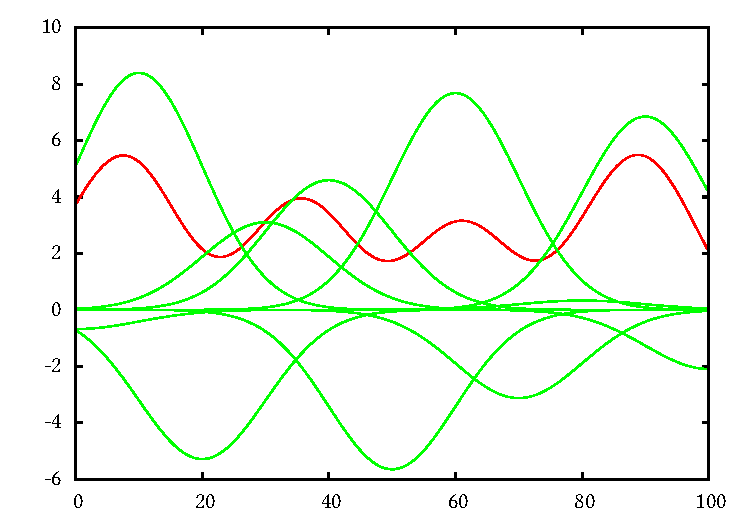
\includegraphics[width=0.5\textwidth]{images/contrib1}
   }
   \subfloat{
   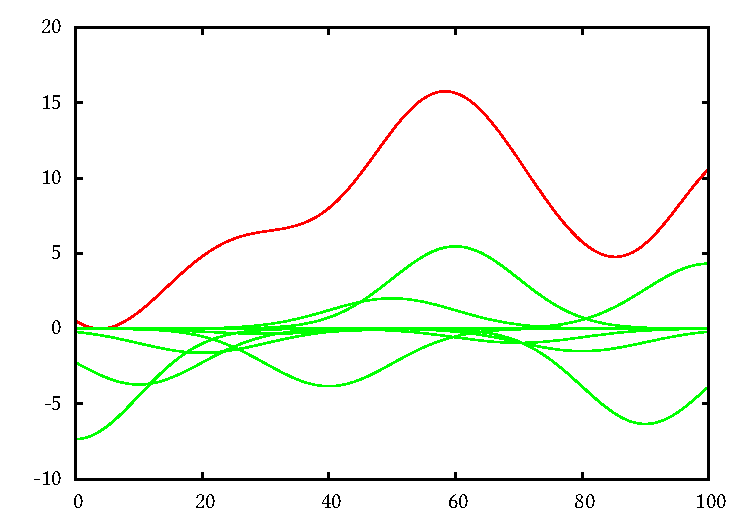
\includegraphics[width=0.5\textwidth]{images/contrib2}
   }
   \caption{Two examples of functions randomly generated from Gaussians. The red
   function is constructed by summing the green gaussians. Generated with
   $\Delta t=$ 10, $\alpha=$ 1. The functions are shifted so that all points
   are $\geq$ 0.}
   \label{fig:contrib}
   \end{figure}
\subsection{Generating Streams from Functions}
\label{sec-3-2}

   Once a function has been generated, we can use it as the rate function
   $\lambda(t)$ for a NHPP, which we can then use to generate event arrival
   times by building on the generation of event times from a HPP.

   We use inverse transform sampling to generate event times from a HPP. This
   technique works by generating a uniform random number $U\sim U(0,1)$, and
   finding the value on the $x$-axis at which the cumulative distribution
   function (CDF) of a probability distribution is equal to the value of $U$. To
   do so, it is necessary to invert the CDF. The waiting time to the next event
   in a Poisson process is an exponential function, which has CDF $1-e^{\lambda
   x}$, which we can invert using the $\log$ function, giving us the
   waiting time $t$ to the next event as \cite{1998art}
   \begin{align}\label{eq:homlambda}
   t=-\frac{1}{\lambda}\log(U)
   \end{align}
   Using this calculation, it is possible to generate a realisation of a HPP for
   an interval of any finite length. This provides a base which can be extended
   to generate events from NHPPs.
   
   To generate events from an NHPP with a rate function $\lambda(t)$, we use a
   technique called thinning, where we generate a large number of values, and
   then throw some of them away based on some criterion. In the case of the
   NHPP, we generate events from a HPP with a rate parameter $\lambda$, where
   $\lambda>\lambda(t)$ for $0<=t<=T$. In other words, the homogeneous lambda
   value must be larger than the value of the rate function for the whole time
   the process runs. First, two random values are independently sampled from a
   uniform distribution, $U_1,U_2\sim U(0,1)$. The first number, $U_1$, is used
   in \eqref{eq:homlambda} to find the next event time from the homogeneous
   process governed by $\lambda$. Using the time $t$ generated from that, the
   value of $\lambda(t)$ is calculated. If $U_2\leq\frac{\lambda(t)}{\lambda}$,
   then the event is kept. The closer $\lambda(t)$ is to $\lambda$, the more
   events will be kept, and so the number of events generated depends on the
   shape of the rate function.
\section{Function Estimation}
\label{sec-4}

  Once we have a photon stream, the next stage is to estimate its characteristic
  function. This section presents the two methods that we implemented to do
  this. The first method uses simple linear regression, and the second a kernel
  density estimator.
\subsection{Baseline Estimation}
\label{sec-4-1}

   In this section, we present the baseline method for function estimation. The
   core of the estimator is based on the iterative weighted least squares
   estimator derived by Massey et.al \cite{massey1996estimating}, and in the
   next two sections we attempt to explain it in simple terms. The subsequent
   sections detail our additions to the simple estimators in order to form the
   final baseline estimator.
\subsubsection{Ordinary Least Squares}
\label{sec-4-1-1}

    The ordinary least squares (OLS) estimator forms the core of the baseline
    estimator, estimating functions by minimising the sum of squared
    residuals. It is important to note the difference between errors and
    residuals. In statistical terms, an \emph{error} is ``The difference between
    the observed value of an index and its ``true'' value'' \cite{2008oecd}, and
    a \emph{residual} is ``The difference between the observed value of a
    response variable and the value predicted by some model of interest''
    \cite{everitt2010cambridge}. The true value of the function is
    unobservable---it is only possible to obtain a statistical sample. The
    residual, on the other hand, is the difference of the observation from some
    \emph{estimate} of the function. This first estimator estimates a linear
    function of the form $y=ax+b$, or a straight line. While this is not
    directly useful for estimating characteristic functions, it was developed in
    order to gain a deeper understanding of the ideas behind regression, and we
    will extend it for our purposes in later sections.

    In order to estimate the function, the stream of event times must first be
    converted into a form which is suitable for processing. To do this, we first
    pick a time interval $(0,T]$, and divide it into $N$ sub-intervals, or
    \emph{bins}. According to \cite{massey1996estimating}, the $k\text{th}$ bin
    $I_k$ is calculated by
    \begin{align}
    I_k&=\left(\frac{(k-1)T}{N}, \frac{kT}{N}\right],\,1\leq k\leq N
    \intertext{and the midpoint $x_k$ of each bin is}
    x_k&=\left(k-\frac{1}{2}\right)\frac{T}{N},\,1\leq k\leq N
    \end{align}
    Due to the independent increments property of Poisson processes, splitting
    the interval leaves us with $N$ bins, each of which is defined by an
    independent Poisson random variable \cite{massey1996estimating} $Y_k$ with
    mean
    \begin{equation}\label{eq:lam}
    {\lambda}_k=\frac{T}{N}(a+bx_k)
    \end{equation}
    where $T/N$ is used to normalise the value of ${\lambda}_k$. The value of
    $Y_k$ in our case is the number of photon arrival times for each bin. In
    order to perform regression on the data, we need a model, which is used to
    connect the random variables and the parameters, and describes how they are
    related. Our model becomes $Y=\alpha+\beta x +\epsilon$, or     $Y_k=\alpha+\beta x_k + \epsilon_k$ \cite{massey1996estimating}. The values
    $\alpha$ and $\beta$ are the two regression parameters which we use to
    estimate the values of $a$ and $b$ in the characteristic function. We
    introduce a Poisson error $\epsilon$ which represents the error present in
    the data that we are trying to model. As mentioned before, this technique
    works by minimising the sum of squared residuals. The square of a residual
    can be computed by \cite{kenney1962mathematics}
    \begin{equation}\label{eq:sqres}
    d_k^2=(Y_k-[\alpha +\beta x_k])^2
    \end{equation}
    We use the regression parameters $\alpha$ and $\beta$ rather than the
    unknowable values $a$ and $b$, since we calculate residuals in relation to
    the estimate of the function. We introduce a weight $w_k$, initialised to 1,
    for each interval, which compensates for the Poisson error
    \cite{massey1996estimating}. Introducing this weight into \eqref{eq:sqres}
    and summing over all bins, we compute a weighted version of the residual sum
    of squares (RSS). We want to find the values of $\alpha$ and $\beta$ for
    which the RSS is minimised.
    \begin{equation}
    \arg\min_{\alpha,\beta}\sum_{k=1}^N w_k(Y_k-[\alpha +\beta x_k])^2
    \end{equation}
    This is known as the \emph{objective function}. Once the objective function
    is known, we can define estimators $\hat{\alpha}$ and $\hat{\beta}$, which
    we will use to estimate values of $\alpha$ and $\beta$ to find the minimum
    \cite{massey1996estimating}.
    \begin{equation}
    \hat{\beta}
    =\frac{\displaystyle\sum_{k=1}^N w_k(x_k-\bar{x})(Y_k-\bar{Y})}{\displaystyle \sum_{k=1}^N w_k(x_k-\bar{x})^2}
    =\frac{\displaystyle\sum_{k=1}^N w_k(x_k-\bar{x})Y_k}{\displaystyle\sum_{k=1}^N w_k(x_k-\bar{x})^2}
    \end{equation}

    \begin{equation}
    \hat{\alpha}=\bar{Y}-\hat{\beta}\bar{x}
    \end{equation}

    \begin{equation}
    \text{where}\quad
    \bar{x}=\frac{1}{N}\sum_{k=1}^N w_kx_k\quad \text{and}\quad
    \bar{Y}=\frac{1}{N}\sum_{k=1}^N w_kY_k
    \end{equation}

    If we ignore the effect of adding the weight $w_k$ for the time being, the
    calculation of $\hat{\beta}$ is equivalent to dividing the covariance of $x$
    with $Y$ by the variance of $x$ \cite{kenney1962mathematics}. The covariance
    is a measure of the strength of the correlation between two or more random
    variables \cite{covariance}. If high values of one variable occur when the
    other variable also has high values, then the covariance is positive. If
    high values of one variable occur when the other has low values, then it is
    negative. The variance, on the other hand, is a measure of the variation in
    values of a random variable. If all values are close to the mean, then the
    variance is small, and if there are large deviations from the mean value,
    then the variance is large. If the covariance is positive, then the values
    of $Y$ increase as $x$ increases. The variance of $x$ depends only on the
    length of the interval---short intervals have low variance, and long
    intervals high variance. This is because the calculation of the variance is
    done by finding the distance to the midpoints of bins from the value of
    $\bar{x}$, which is the midpoint of the interval.
    
    It is clear that the sign of $\hat{\beta}$ depends on whether the covariance
    is positive or negative, and this in turn defines the sign of the
    gradient. The steepness of the gradient is defined by the magnitude of the
    covariance. Since the value of the variance is constant, the larger the
    magnitude of the covariance, the steeper the gradient. Once we know the
    gradient of the line, the calculation of the intercept is simple, so long as
    we know the value of a point on the line. The point $(\bar{x},\bar{Y})$ is
    one such point. We rearrange the equation
    $\bar{Y}=\hat{\alpha}+\hat{\beta}\bar{x}$ to solve for
    $\hat{\alpha}$. Notice that since the values of $\bar{x}$ and $\bar{Y}$ do
    not change, the line estimate pivots around the point defined by the mean
    values. The addition of the weights adds bias into the calculation, taking
    into consideration the variation of those bins which have a smaller
    estimated value of $\lambda$. The weight update calculation is discussed in
    the next section.

    We normalise the values of $\hat{\alpha}$ and $\hat{\beta}$ by multiplying
    the resulting estimate by the number of bins over the interval length. The
    fewer bins used in the estimate, the larger the bin count will be for each
    bin, and consequently the larger the estimated values will be. To return the
    estimate to the correct scale, we set
    \begin{equation}
    \hat{a}=\frac{N}{T}\hat{\alpha}\quad\text{and}\quad
    \hat{b}=\frac{N}{T}\hat{\beta}
    \end{equation}
    As we are dealing with a Poisson process with a rate function, it is natural
    to impose a constraint on the values of $\hat{a}$ and $\hat{b}$ which states
    that the rate function must be non-negative throughout the entire interval
    $[0,T]$, since it is not possible to have a negative rate
    \cite{massey1996estimating}.
    \begin{equation}
    \hat{a}\geq 0\quad \text{and}\quad
    \hat{b}\geq -\hat{a}/T
    \end{equation}
    There are two cases in which this constraint can be violated; when $a<0$ or
    $b<-\hat{a}/T$ \cite{massey1996estimating}. In the first case, we set
    \begin{align}
    \begin{split}
    \hat{a}&=0\\
    \hat{b}&=\frac{N}{T}\frac{\displaystyle \sum_{k=1}^N w_kx_kY_k}{\displaystyle\sum_{k=1}^N w_kx_k^2}
    \end{split}
    \end{align}
    and in the second,
    \begin{align}
    \begin{split}
    \hat{a}&=-\hat{b}T\\
    \hat{b}&=-\frac{N}{T}\frac{\displaystyle \sum_{k=1}^N (T-x_k)Y_k}{\displaystyle \sum_{k=1}^N w_k(T-x_k)^2}
    \end{split}
    \end{align}
    Applying these adjustments in the cases in which the constraints are
    violated ensures that the final estimate is always within the required
    constraints. However, the adjustments introduce some non-linearity into the
    system \cite{massey1996estimating}. With this set of equations, the
    fundamental structure of the OLS estimator is complete. In the next section,
    we discuss the addition of weight update rules and finding estimates of
    $\lambda$.
\subsubsection{Iterative Weighted Least Squares}
\label{sec-4-1-2}

    \begin{figure}[h]
    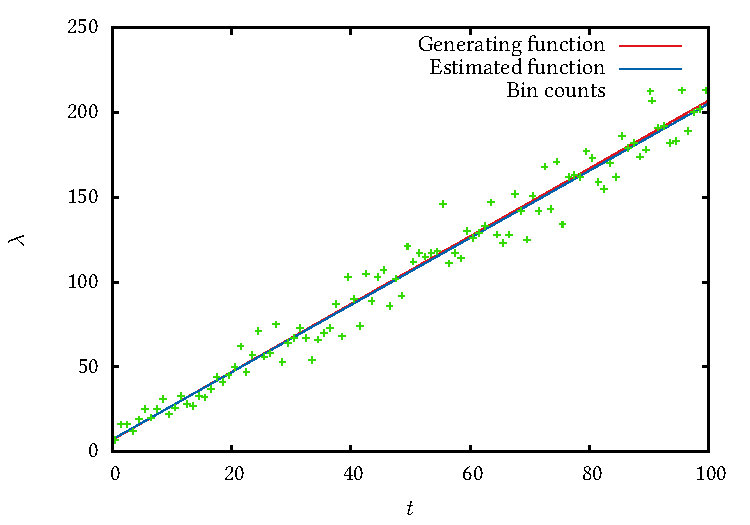
\includegraphics{images/lineest}
    \caption{IWLS estimate of a photon stream with the characteristic function
    $\lambda(t)=a+bt$ where $a=$ 7 and $b=$ 2.}
    \label{linefig}
    \end{figure}
    The iterative weighted least squares (IWLS) estimator builds upon the OLS
    estimator. As the name suggests, the extension introduces an iterative
    part. The OLS estimator performs a single estimate of the function, whereas
    IWLS estimator repeats the process multiple times, updating its estimates
    each time.

    Perhaps the most important update to the estimator is the use of unequal
    weights, which change depending on the variances of the random variable
    which defines the bin which the weight is being applied to. A Poisson random
    variable has a variance that is equal to its mean---this means that a higher
    value of $\lambda$ results in a larger variance. To compensate for this,
    we give higher weights to bins which have lower values of $\lambda$, as the
    variances will be lower. As shown in equation \eqref{eq:lam}, the value of
    $\lambda$ is easy to calculate, but the values of $a$ and $b$ must be
    known. In order to modify weights appropriately, we must be able to obtain
    estimates of $\lambda$, which can be done using \cite{massey1996estimating}
    \begin{align}
    \hat{\lambda}_k=\frac{T}{N}(\hat{a}+\hat{b}x_k)
    \end{align}
    The weights can then be updated by
    \begin{equation}
    \hat{w_k}=\frac{\displaystyle \frac{N}{\hat{\lambda}_k}}{\displaystyle \sum_{k-1}^N\left(\frac{1}{\hat{\lambda}_k}\right)}
    \end{equation}
    Each iteration of the estimator updates these estimates of $\lambda$ and the
    weight for each bin, and the process is stopped when the change in the
    estimates becomes negligible, which consistently happens in between two and
    five iterations \cite{massey1996estimating}. Figure \ref{linefig} shows an
    example of a function estimated using IWLS.

    While this is an improvement on the OLS estimator, it is not sufficient for
    our purposes. The characteristic functions of stellar objects are not
    straight line functions, so we must extend this approach to give us some
    reasonable estimates of functions which are not straight lines.
\subsubsection{Piecewise Iterative Weighted Least Squares}
\label{sec-4-1-3}

    It is clear that the IWLS estimator alone is not sufficient to complete our
    task. In order to obtain a reasonable estimate of the characteristic
    function, we need to be able to estimate a function which is not a straight
    line. During the development process, we considered the possibility of
    approximating functions by multiple straight-line estimates, and this
    estimator is the result. This type of function is known as a piecewise
    linear function. Extending the approach presented in the previous two
    sections, we take the interval $[0,T]$, and split it into several
    sub-intervals. Then, the function underlying each of these sub-intervals is
    estimated using IWLS. We also add some minor extensions in an attempt to
    improve the quality of the estimates.

    Sub-intervals are estimated starting from the first, and moving to the next
    once the process is complete. When the estimate is completed, a short
    interval after the sub-interval being estimated is checked to see how well
    the estimate for the previous sub-interval matches it. The extension
    interval is split into several bins. Using a probability density function
    (PDF), we evaluate the likelihood of obtaining the count $Y_k$ for each bin
    given the estimate $\lambda$ at that point. The PDF for a Poisson
    distribution is calculated by
    \begin{equation}
    P(Y_k=x)=\frac{\lambda^xe^{-\lambda}}{x!}
    \end{equation}
    
    For each bin, $P(Y_k=x)$ must exceed some threshold. A lower threshold means
    that lines are less likely to be successfully extended. While this technique
    is an improvement on using straight lines to estimate functions which are
    curves, it is still not sufficient, as the resulting function estimate is
    piecewise disjoint---the estimate for each interval does not connect
    smoothly into the next, but jumps at the boundary between each sub-interval.
    \begin{figure}[h]
    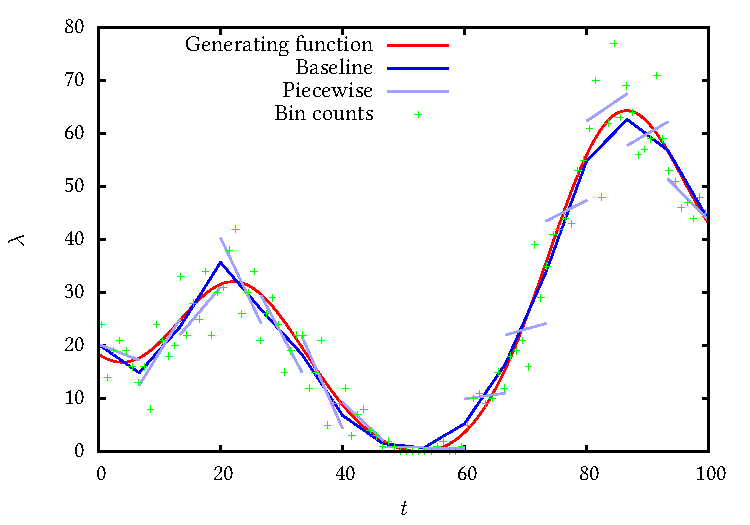
\includegraphics{images/pcbase}
    \caption{A comparison of the baseline and piecewise estimates on the same
    function. Note how the baseline estimate passes through the midpoint of the
    disjoint piecewise estimates at the breakpoints.}
    \label{fig:basecomp}
    \end{figure}
\subsubsection{Baseline}
\label{sec-4-1-4}

    As mentioned in the previous section, the piecewise IWLS estimator gives us
    a piecewise disjoint estimate of the function, but we would like one which
    is piecewise continuous. In order to do this, the end of each interval
    estimate must meet the start of the next. The estimate returned by the
    piecewise estimator has several breakpoints---points where the start of one
    sub-interval and the end of another meet. If there are $L$ lines that make
    up the estimate, there will be $R=L-1$ breakpoints. At each of these
    breakpoints $r$, we calculate the value of the previous and subsequent
    function estimates $f$, and find their midpoint $m$ with
    \begin{equation}
    m_i = \frac{f_{i}(r_i) + f_{i+1}(r_i)}{2},\quad 0\leq i < R
    \end{equation}
    The value of $m$ is calculated for each breakpoint. Midpoints are not
    calculated at time 0 and time $T$. Instead, the function values at those
    points are used. Each sub-interval is now represented by a point $p$ at the
    start and $q$ at the end, each with an $x$ and $y$ coordinate. With these
    points, we can recalculate each sub-interval estimate $f$ of the form
    $y=\hat{a}+\hat{b}x$ by replacing $y$ with $p_y$ and $x$ with $p_x$, and
    recalculating the gradient $\hat{b}$ and intercept $\hat{a}$ with
    \begin{align}
    \hat{b} &= \frac{q_y-p_y}{q_x-p_x}\\
    \hat{a} &= p_y - \hat{b}\cdot p_x
    \end{align}
    In this way, each sub-interval estimate links points $p$ and $q$, giving us
    a piecewise continuous function estimate, and this step completes the first
    function estimation method. Figure \ref{fig:basecomp} shows an example of a
    piecewise and baseline estimate.
\subsection{Kernel Density Estimation}
\label{sec-4-2}

   The second function estimation method implemented was a kernel density
   estimator, which use \emph{kernels} to estimate the probability density of a
   random variable. A kernel is simply a weighting function, which affects how
   much a given sample is considered when constructing the function
   estimate. Since the photon stream data is assumed to be generated by a source
   whose variability is defined by some random variable, the event times are a
   sample drawn from the PDF of that variable. We use a Gaussian kernel
   \begin{align}
   K(t,\mu)=e^{-(t-\mu)^2/2\sigma^2}
   \end{align}
   to estimate the PDF, centring a kernel at each photon arrival time $a$ by
   setting $\mu=a$. The width of the kernel depends on some fixed value
   $\sigma$. We perform a Gauss transform on the $N$ kernels, finding the
   contribution of all the kernels at $M$ points in time, from which we get an
   estimate $\hat{\lambda}(t)$ of the characteristic function.
   \begin{align}
   \hat{\lambda}(t_i) = \sum_{j=1}^N K(t_i,\mu_j), \quad i=1,\dots,M
   \end{align}
   Using a larger $M$ gives a higher resolution. Depending on the value of
   $\sigma$ used, $\hat{\lambda}(t)$ will be some multiple of the actual
   function $\lambda(t)$. Thus, the final step is to normalise
   $\hat{\lambda}(t)$. We split the stream data into $B$ bins with midpoints $b$
   and calculate the bin count $x$ for each. We start with the normalisation
   constant $\eta$ at a low value, and gradually increase it to some threshold,
   finding
   \begin{equation}\label{eq:normcalc}
   \sum_{i=1}^B
   \log\left(\frac{\phi^xe^{-\phi}}{x!}\right), \quad \phi=\eta\cdot\hat{\lambda}(b_i)
   \end{equation}
   for each value of $\eta$. The value of $\eta$ which maximises this sum of log
   Poisson PDFs is used to normalise $\hat{\lambda}(t)$ in subsequent
   computations. Figure \ref{fig:kde} shows an example of a kernel density
   estimate, and displays a weakness in the estimator. As one moves towards the
   start or end of the interval, fewer Gaussians make a noticeable contribution
   to the function calculation, resulting in a drop-off of the estimate.
   \begin{figure}[h]
   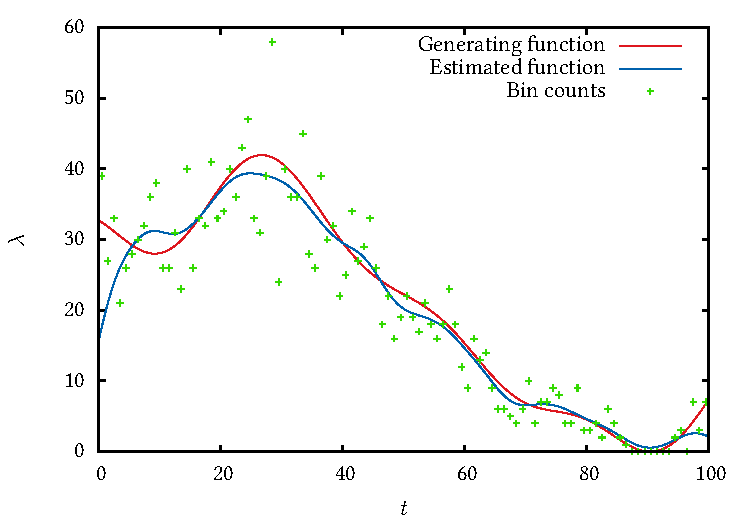
\includegraphics{images/gauss}
   \caption{Estimate of a function using Gaussian kernels. The drop-off at the
   start and end of the interval is due to fewer Gaussians summed in those areas
   as no kernels are placed outside the interval.}
   \label{fig:kde}
   \end{figure}
\section{Time Delay Estimation}
\label{sec-5}

  Once we are able to estimate the characteristic function of photon streams, we
  can use these estimates to compute an estimate of the time delay between two
  streams. If the two streams come from the same source, then they should have
  the same characteristic function, but delayed by some value $\Delta$. Our
  estimates of the characteristic function will differ for both streams due to
  the fact that the number of photon arrivals in each bin will be different for
  each stream, but each should look relatively similar. In this section we
  present two methods for estimating the time delay between a pair of streams
  based on their function estimates.

  Both of the estimators work by starting $\Delta$ at $-\Delta_{\text{max}}$,
  and increment it by some step until $+\Delta_{\text{max}}$ is reached,
  using a metric to evaluate how good the estimate is with that value. It is
  important to note that the value of $\Delta_{\text{max}}$ defines the interval
  in which the metric is computed. The need for calculation only in some
  specific interval should be clear---if one function is shifted by $\Delta$,
  and both functions have the same time interval, then there will be an interval
  of length $\Delta$ at either end of the range in which only one of the
  function estimates has values. As such, the metric can only be computed in the
  overlapping area. Varying $\Delta$ changes the overlapping interval. Setting
  $\Delta=0$ minimises the value, and $\Delta=\pm\Delta_{\text{max}}$ maximises
  it. Performing calculations on different interval lengths would require the
  value of the metric for longer intervals to be scaled to that of the
  shortest. To make useful comparisons, we must perform calculations only on the
  interval in which the two functions overlap for all values of
  $\Delta$. Imposing this constraint means that the value of
  $\Delta_{\text{max}}$ can never exceed the interval length $T_{\text{est}}$ in which we are
  performing the estimate. We are left with the constraints
  $T_{\text{est}}=[t_0+\Delta_{\text{max}},
  T-\Delta_{\text{max}}],\,\Delta_{\text{max}}<T$ on the interval and the
  maximum value of $\Delta$.
\subsection{Area Method}
\label{sec-5-1}

   The first of the two methods uses a very simple metric to estimate the time
   delay. By taking the two function estimates, we can attempt to match up the
   two functions so that they ``fit together'' best. The goodness of fit can be
   determined by the area between the two functions $\hat{\lambda}_1$ and
   $\hat{\lambda}_2$, calculated by
   \begin{align}
   \begin{split}
   d(\hat{\lambda}_1,\hat{\lambda}_2)&=\int(\hat{\lambda}_1(t)-\hat{\lambda}_2(t+\Delta))^2\,dt\\
   &\approx\frac{1}{N}\sum_{i=1}^N(\hat{\lambda}_1(t)-\hat{\lambda}_2(t+\Delta))^2
   \end{split}
   \end{align}
   for each value of $\Delta$. Our estimate of $\Delta$ is set to the value at
   which $d(\hat{\lambda}_1,\hat{\lambda}_2)$ is minimised. Rather than using an
   integral to get the exact area between the functions, we use a less
   computationally expensive discrete approximation. Figure \ref{fig:areamethod}
   shows a visual representation of the logic behind the method.
   \begin{figure}[h]
   \subfloat[High area ($\Delta=$ 0)]{
   \includegraphics[width=0.5\textwidth]{images/normarea}
   %\includegraphics{normarea}
   }
   \subfloat[Low area ($\Delta=$ 13.3)]{
   \includegraphics[width=0.5\textwidth]{images/shiftarea}
   %\includegraphics{shiftarea}
   }
   \caption{Comparison of area between functions for two different values of
   $\Delta$. The first 13.3 time units must be ignored in (b). The value of
   $\Delta$ in (b) clearly results in a closer match and lower area between the two functions
   than the value in (a).}
   \label{fig:areamethod}
   \end{figure}
\subsection{Probability Density Function Method}
\label{sec-5-2}

   The second method of estimation is using probability density functions. As
   before, we guess a value of $\Delta$ between $-\Delta_{\text{max}}$ and
   $+\Delta_{\text{max}}$ and shift $\hat{\lambda}_2$ by that amount. However,
   we know that there must be a single characteristic function, and we want to
   see how well our estimate of that matches the bin counts in each stream. We
   make an ``average'' function $\bar{\lambda}$ by combining the two function
   estimates we have, $\hat{\lambda}_1$ and $\hat{\lambda}_2$ (which is shifted
   by $\Delta$).
   \begin{equation}
   \bar{\lambda}(t)=\frac{\hat{\lambda}_1(t)+\hat{\lambda}_2(t+\Delta)}{2}
   \end{equation}
   The point on $\bar{\lambda}$ at time $t$ is the midpoint between the values of
   the two estimates at that time. Once we have $\bar{\lambda}$, we can assign some
   score to the current estimate of the value of $\Delta$.
   \begin{align}
   \begin{split}
   \log P(S_A,S_B\mid\bar{\lambda}(t))=\sum_{t=\Delta_{\text{max}}}^{T-\Delta_{\text{max}}}&\log P(S_A(t)\mid \bar{\lambda}(t))\\
   &+ \log P(S_B(t+\Delta)\mid \bar{\lambda}(t))\\
   \end{split}
   \end{align}
   Here, we calculate the probability that the function $\bar{\lambda}$ is the
   characteristic function of the two streams $S_A$ and $S_B$. The streams are
   split into bins, and the log probability of the number of events in each bin
   given the value of $\lambda$ calculated for that bin is computed and summed
   over all bins, as in Equation \eqref{eq:normcalc}.

   The calculation of $\lambda$ is slightly more complicated than just taking
   its value at the midpoint of each bin. Since we are considering a number of
   events occurring in a given interval, we must consider the value of $\lambda$
   for the same interval. In order to do this, we use a discrete approximation
   of integrating $\lambda(t)$ over the interval.
   \begin{align}
   \lambda_{a,b}&=\int_a^b\lambda(t)\,dt
   \end{align}
   In the approximation $t$ is incremented by some finite step for each
   successive value. The smaller the value of the step the more accurate the
   approximation of $\lambda_{a,b}$ becomes. As with the previous estimator, the
   estimate is made in two stages, first with a coarse pass over the values of
   delta to compute an initial estimate, and then a finer second pass around the
   first estimated value in order to refine the estimate. Figure
   \ref{fig:finest} illustrates the whole estimation process.
   \begin{figure}[h!]
   \subfloat[Estimate functions based on bin data]{
   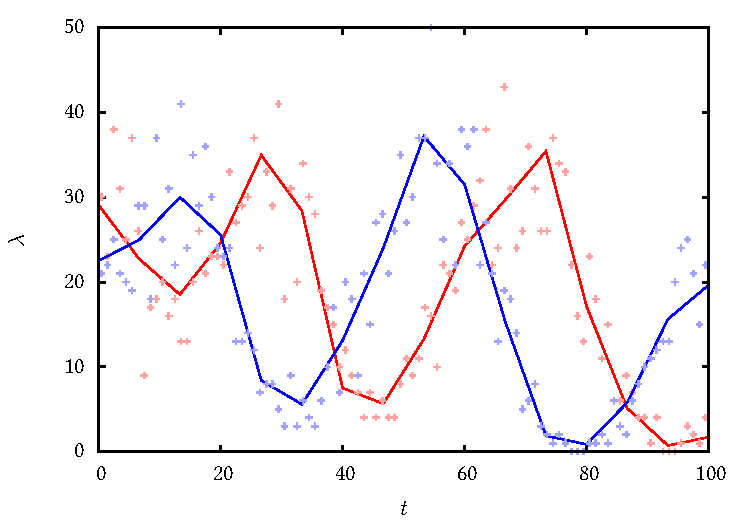
\includegraphics[width=0.5\textwidth]{images/baseest}
   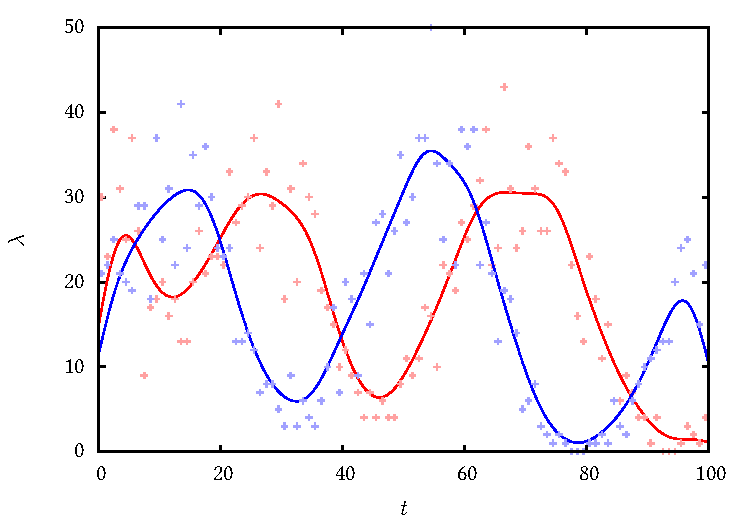
\includegraphics[width=0.5\textwidth]{images/gaussest}
   }\\
   \subfloat[Shift second (blue) function based on $\Delta$ estimate]{
   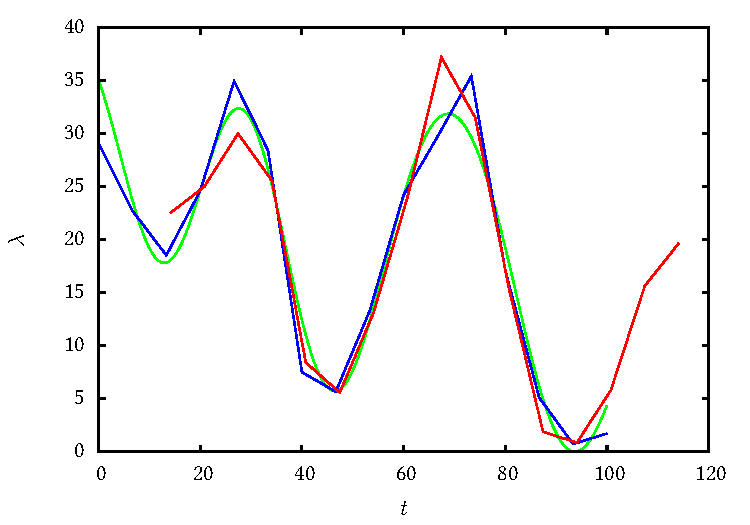
\includegraphics[width=0.5\textwidth]{images/baseshift}
   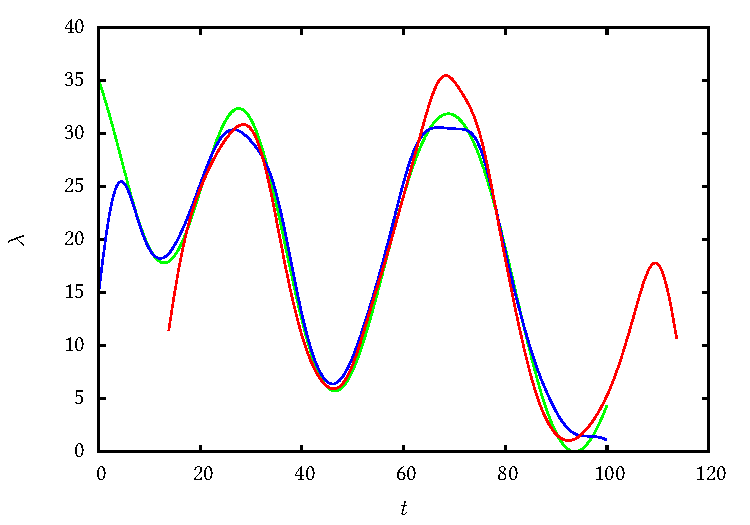
\includegraphics[width=0.5\textwidth]{images/gaussshift}
   }\\
   \subfloat[Combine functions to create final estimate]{
   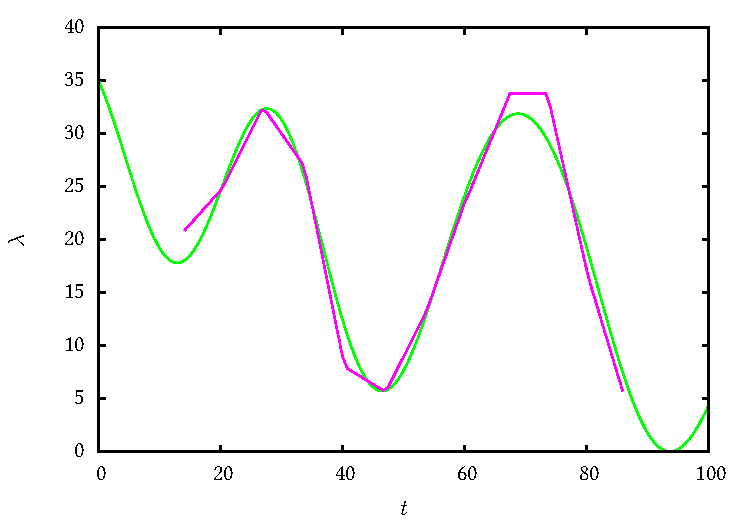
\includegraphics[width=0.5\textwidth]{images/basecomb}
   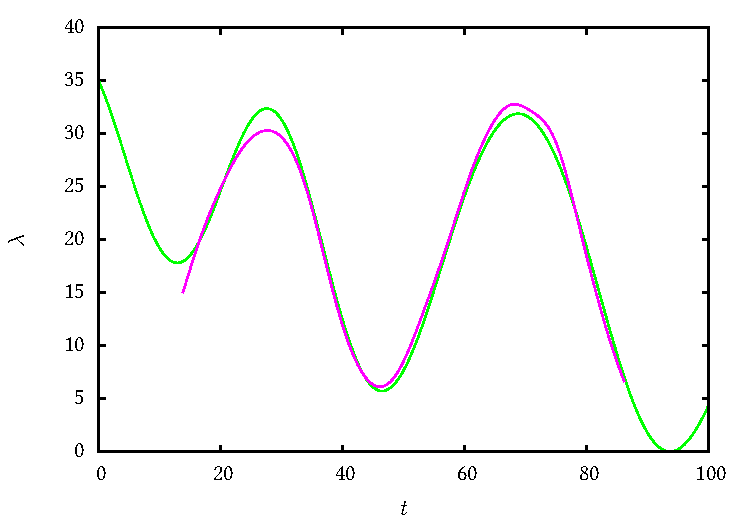
\includegraphics[width=0.5\textwidth]{images/gausscomb}
   }
   \caption{Illustration of the estimation process. Left column shows baseline
   method, right column Gaussian. The estimated value of $\Delta$ was 14.1 and
   13.8 for baseline and Gaussian respectively, found using the PDF
   method. Actual value was 15.  Points in (a) represent bin counts for the
   function of the same colour. The green line in (b) and (c) indicates the actual function,
   magenta is the final estimate.}
   \label{fig:finest}
   \end{figure}
\section{System}
\label{sec-6}

  In this section we provide an overview of the system, and explain some of the
  details behind the implementation of the system. We also give some idea about
  the design decisions used in the implementation. Discussion of the programming
  methodologies and ideas used can be found in the \ref{sec-7} section. The
  system is very large (over 7000 lines of C code), and we therefore attempt to
  detail the key ideas behind each part of the implementation rather than an in
  depth discussion of the techniques. Each subsystem described in sections
  \ref{sec-3}--\ref{sec-5} also has its own section
  describing some of the important parts of its implementation.
\subsection{Design}
\label{sec-6-1}

   When designing the system, we made the decision to split the three main
   pieces of required functionality into two groups. The generation of streams
   and functions would make up one subsystem, and the function and time delay
   estimation would make up another. This is a logical way in which to divide
   the system, as they are linked only by the dependence of the estimators on
   data from the generators. It is not strictly necessary for the data to come
   from inside the system---as long as it has the structure required by the
   estimators it can be used. We use a single executable to launch both of the
   subsystems. Figure \ref{fig:sysstruct} gives an overview of the structure of
   the system.

   As with any large program, there will inevitably be some code which has to be
   used in different places in the program. To make checking the correctness of
   the system and its modification easier, functions that are called more than
   once are put into libraries which are shared between all subsystems.

   The input and output of the system is another important thing that must be
   considered. The system should be able to read data which follows some sort of
   structure. The structure should be simple, so that minimal effort is required
   to convert data into a form which the system can process. Input to the system
   is from simple text files, which are easy to construct, and easy to read
   in. Output from the system, both in terms of output to the interface, and
   also output files, also need to have some meaningful structure, and the
   results of calculations should be clear. Output files should not contain any
   unneeded information. The system can be made to output more detailed data, or
   not output anything at all, with the use of output flags. Output filenames
   are highly structured, which make reading in data much easier, and is of
   particular importance when doing experiments.

   Once parameters are set, user interaction with the program is minimal. The
   output of the system is all numerical data. Textual output is simple to
   display, and there are many utility programs that can parse data files to
   draw graphs. As such, we decided not to use a command line interface over a
   graphical one. The development of a graphical interface is time consuming,
   and requires a lot of thought to be put into design. On the other hand,
   interaction with the command line is simply a question of reading text
   responses or parsing command line options. A graphical interface for the
   system would provide little benefit to the user in terms of additional
   information, as the system is a tool to use for data processing, not
   something that requires constant interaction with the user. Most scientists
   interact regularly with computers, and astronomers in particular regularly
   use data processing programs. As our intended user base is likely to have
   experience with command line interfaces, we feel that the lack of a graphical
   interface does not reflect negatively on the system.

   In order to test the various methods developed, there has to be a way of
   running controlled experiments on the system. For this purpose, an experiment
   system which is a wrapper around the estimators forms the final
   subsystem. With it, multiple calls to the estimators can be made with
   different configuration parameters.

   In addition to the core of the system, scripts are provided which can be used
   to plot the output data, and run more complex sets of
   experiments. Usage instructions can be found in Appendix \ref{sec-10-3} and \ref{sec-10-2-4}.
   \begin{figure}
   \centering
   \pgfdeclarelayer{background}
   \pgfdeclarelayer{foreground}
   \pgfsetlayers{background,main,foreground}
   % horizontal separation
   \def \hnsep {0.5}
   \tikzstyle{sub}=[draw, fill=blue!20, text width=5em, 
   text centered, minimum height=2.5em, node distance=1.5cm]

   \begin{tikzpicture}
   \node (param) at (2,3) [sub] {Parameter file};
   % libs group
   \node (lib) at (6,3) [sub] {Libraries};
   % generator group
   \node (gen) at (2,0) [sub] {Generators};
   \node (strout) [sub, below of=gen] {Stream Data};
   % estimator group
   \node (est) at (6,0) [sub] {Estimators};
   \node (estout) [sub, below of=est] {Estimator Output};
   % experimenter
   \node (expparam) at (10,3) [sub] {Experiment Parameters};
   \node (explbl) at (10,0) [sub] {Experiment};
   \node (expout) [sub, below of=explbl] {Experiment Results};
   % launcher
   \node (launcher) at (0,1.5) [sub] {Launcher};
   % Draw the rest on the background layer
   \begin{pgfonlayer}{background}

   % path from expparam to experiments
   \coordinate [above=0.5 of explbl] (expln) {};
   \coordinate [below=0.8 of expparam] (exppjoin) {};
   \draw [line width=1pt] (expparam.south) -| (exppjoin);
   % path from experiments to exp out
   \draw [dashed,->,line width=1pt] (explbl.south) -- (expout.north);

   % launcher arrows
   \path (est.north)+(-0.3,-0.13) node (estla) {};
   \draw [->,line width=1pt,red] (launcher.east) -| (estla);
   \path (gen.north)+(-0.3,-0.13) node (genla) {};
   \draw [->,line width=1pt,red] (launcher.east) -| (genla);
   \path (explbl.north)+(-0.3,-0.13) node (expla) {};
   \draw [->,line width=1pt,red] (launcher.east) -| (expla);

   % library arrows
   \path (est.north) node (esttop){};    
   \coordinate [above of=gen] (gentop) {};
   \coordinate [below=0.8 of lib] (lsplit) {};
   \draw [-,line width=1pt] (lib.south) -- (lsplit);
   \draw [->,line width=1pt] (lsplit) -- (est.north);
   \draw [->,line width=1pt] (lsplit) -| (explbl.north);
   \draw [->,line width=1pt] (lsplit) -| (gen.north);

   % path from param to library link
   \coordinate [above=0.5 of lsplit] (tt) {};
   \coordinate [right=0.5 of param.east] (pright) {};
   \draw [line width=1pt] (param.east) -- (pright);
   \draw [line width=1pt] (pright) |- (tt);

   % estimator arrows
   \draw [dashed,->,line width=1pt] (est.south)--(estout.north);
   \coordinate [right=0.9 of estout] (restout) {};
   \coordinate [above=0.5 of explbl] (abvexp) {};
   \draw [line width=1pt] (estout.east) -- (restout);
   \draw [line width=1pt] (restout) |- (abvexp);

   % generator arrows
   \coordinate [above=0.5 of est] (abvln) {}; %above length est
   \coordinate [right=0.9 of strout] (rstrout) {};
   \draw [dashed,->,line width=1pt] (gen.south) -- (strout);
   \draw [line width=1pt] (strout.east) -- (rstrout);
   \draw [line width=1pt] (rstrout) |- (abvln);

   \end{pgfonlayer}
   \end{tikzpicture}
   \caption{A simplified overview of the system structure. Solid lines indicate
   the dependencies of a given subsystem, and Dashed lines indicate output from a
   subsystem. The red lines indicate what the user can access through the launcher.}
   \label{fig:sysstruct}
   \end{figure}
\subsection{Parameter Files}
\label{sec-6-2}

   The parameter files are used to configure the values of all parameters which
   affect the behaviour of the system. Separate files are used to configure the
   estimators and generators, and the experimenter. The files use a simple
   syntax. The \texttt{\#} symbol defines a comment. A parameter is defined as
   an string of ASCII characters followed by a single space, followed by more
   ASCII characters. Each file is split into several sections, to aid the user
   in finding the parameters they are looking for. All parameters have comments
   describing their effect on the behaviour of the system, what values they can
   take, and other information relevant to the user. Functionality for
   generating parameter files with default settings are provided.
\subsubsection{System File}
\label{sec-6-2-1}

    This parameter file is the one which controls the behaviour of the
    estimators and generators, and is required for almost all operations. It
    facilitates the definition of output filenames, generation parameters for
    the stream generator, including the interval length, start time, and the
    expression used to generate the streams. The random function generator can
    be set up to change the multiplier applied to the Gaussians, change their
    resolution, and define how the standard deviation is set. The configuration
    of all the parameters used by estimators, both function and time delay, is
    also done here. The sections describing the implementation of parts of the
    system explain the exact parameters used and how they affect the behaviour.
\subsubsection{Experiment File}
\label{sec-6-2-2}

    A separate parameter file is used by the experimenter to prevent parameter
    duplication and allow greater flexibility with experiments. It contains
    parameters which affects the naming of output files, and allows the
    configuration of the intervals in which data is withheld in model
    selection. The most important parameters are those which define the names
    and parameters to test during the experiments.
\subsection{Libraries}
\label{sec-6-3}

   The system makes extensive use of custom libraries. Each library consists of
   a header file which contains the function prototypes and include information,
   along with a separate file for the functions, which are compiled by
   \texttt{libtool} into a convenience library. The advantage of using
   \texttt{libtool} over other ways of constructing libraries is that it can
   create both shared and static libraries. This means that if the library needs
   to be re-used elsewhere it is simple to take the shared object file created
   and compile the program including the library by passing the standard
   \texttt{-l[libname]} syntax to \texttt{gcc}. Due to some interdependencies
   between the lower level convenience libraries, they are merged into one main
   library, again functionality provided by \texttt{libtool}. The main purpose
   of the libraries is to provide a single place where oft-used functions can be
   defined once and used by all parts of the system.
\subsubsection{Parameter List}
\label{sec-6-3-1}

    The parameter list library defines a singly-linked list, used to store data
    parsed from the parameter files. These lists are required by many functions
    in the system to set their behaviour. The library provides functions for
    adding elements to the list and finding its length. A function for removal
    of elements is not provided, as there is no situation which should
    necessitate the removal of elements from the list. There is also
    functionality for checking whether a parameter with a given name exists,
    retrieving the value of a parameter, and setting the value of a parameter.

    There are multiple retrieval functions, each of which retrieves values of
    different types. The parameter list is constructed in such a way that all
    values in it are stored as character arrays. This means that if a parameter
    value is required by some function, it must be converted into the type which
    that function requires. Since it is known inside the function which type is
    required, the relevant function can be called. Functions to read
    \texttt{double} and \texttt{int} types are provided, along with a function
    to retrieve the character array. In addition, some of the parameters in the
    files are comma-separated lists of integers or doubles, which must be parsed
    into arrays before they can be used. In order to reduce code duplication,
    the conversion of variables to the correct type is done inside the retrieval
    function.

    Parameters are only parsed when they are required by a function. This
    reduces the complexity of the logic, as it is not necessary to deduce the
    type of the parameter---the function knows what type it requires. It also
    reduces the complexity of the data structure, as only character arrays need
    to be stored. In addition, some parameters are not required by some
    subsystems, so parsing every parameter in the file is unnecessary.
\subsubsection{Mathematics}
\label{sec-6-3-2}

    As the name implies, the mathematics library provides the mathematical
    functions required by the system which are not provided by the standard C
    library. Some of the library functions are based on functionality provided
    by the GNU Scientific Library \cite{gsl}, particularly those which calculate
    probability density functions or require random number generators. The most
    important part of the library is the functionality it provides for
    computations with Gaussians, in particular the discrete Gaussian
    transform. It also provides some basic functions, such as finding the
    minimum and maximum values in arrays, averaging, summing, adding to or
    multiplying arrays, and some implementations of statistical functions such
    as the root mean square error, standard deviation and the like.

    The most challenging part of the implementation of the library was to get
    around the issues caused by double precision values. Functions which deal
    with calculations based on timings require a certain precision on the start
    and end times of intervals to work correctly. Due to the nature of their
    implementation, calculations with doubles often result in numbers which are
    only very close to the actual value. Particular problems were encountered
    when incrementing a value by a floating point number and comparing it to
    another. The floating point increments caused the value to be slightly (on
    the order of \num{1.0e-20}) below the actual value, and this caused
    calculations to be incorrect and resulted in a cascade of erroneous
    calculations. To deal with this problem, functions for comparing doubles to
    a specific precision were implemented.
\subsubsection{Input/Output Utilities}
\label{sec-6-3-3}

    This library implements functionality for reading from and outputting to
    files, as well as for checking the state of files and directories on the
    system. It is also used to parse the parameter file into the system, and as
    such defines the syntax that the parameter file must follow. We were unable
    to find a library which provided similar functionality to the Java
    Properties class, which allows the structured reading and storage of
    parameters, and so implemented a simplified version in the form of the
    parameter files. This library also reads in event data files, which are
    needed as input to the estimators, and can retrieve either all events, or
    data in a specific interval.

    As well as reading in data, the library also serves to output data from
    various data structures used within the system. This ranges from simple
    arrays to more complex data structures used to store representations of
    Gaussians or function estimates.
\subsubsection{General Utilities}
\label{sec-6-3-4}

    The final library is for functions which do not fit in anywhere else, such
    as memory allocation and freeing, printing structs, and error checking
    functions. There are also functions for generating default parameter
    files. This library makes the rest of the system much cleaner, as memory
    allocation and freeing for large structs can be done with a single function
    call. 
\subsection{External Libraries and Tools}
\label{sec-6-4}

   The system uses a number of external libraries to augment the C standard
   libraries, and to reduce the need for us to write code which has already been
   written elsewhere. The GNU Scientific Library \cite{gsl} provides the system
   with a larger variety of random number generators than the standard library
   provides, and also gives access to probability density function
   computations. The Check framework \cite{check} is used to implement automated
   tests for the system, and is part of the GNU build system, which provides
   assistance for making source code packages portable to many Unix systems. Our
   system makes use of the \texttt{automake} and \texttt{libtool} frameworks to
   generate shared library files and makefiles, and directory structure follows
   that of the standard GNU package. The MuParser library \cite{muparser} is
   used to parse expressions used to generate stream data. The Valgrind
   framework was used to debug memory errors \cite{valgrind}.
\subsection{Interface}
\label{sec-6-5}

   Users interact with the system via a command line interface. Various flags
   passed to the executable change the behaviour of the system, but the majority
   of behaviour is controlled through the parameter file. The standard C
   libraries provide a useful function, \texttt{getopt}, specifically for the
   parsing of command line options. This function allows the parsing of short
   options, such as \texttt{-g}, or with the \texttt{getopt\_long} function,
   longer options such as \texttt{--generate} can be parsed. Users familiar with
   *NIX systems will no doubt recognise such options, as they are used in almost
   every program which can be run from the command line. The parsing of options
   is done by the launcher, which is the only part of the system that the user
   interacts with directly. Each subsystem can be run by passing a specific
   option, and checks are made to ensure that only a single subsystem is being
   called. When an error occurs in the parsing of options, which can arise due
   to an option with a required parameter not having anything passed to it, or
   as a result of multiple subsystem calls, an error message is printed
   informing the user of the error.
   
   As with many command line programs, instructions on what options are
   available, and some information on what they do can be displayed using the
   \texttt{-h} or \texttt{--help} options. The help information is also printed
   when there is some issue when parsing the parameters. To better facilitate
   the addition and removal of options, the value of each option is stored as a
   flag in a struct which is used to determine which subsystem to
   run. Instructions on how to use the system can be found in Appendix \ref{sec-10-2}.
\subsection{Function and Stream Generators}
\label{sec-6-6}

   The function and stream generation functions form the \emph{generator}
   subsystem. The two different function generation methods use fundamentally
   different methods to generate functions. The random functions use Gaussians,
   which are represented in a struct containing the mean, standard deviation and
   weight of the Gaussian. We use another struct to store an array of Gaussians
   which represent the whole function. When one of these arrays is generated,
   its constituent Gaussians are output to a file as their mean, standard
   deviation and weight, so they can be used later if necessary. Once one of
   these sets of Gaussians is generated, it is passed to a function which
   implements the thinning procedure. The rate function $\lambda(t)$ is
   generated by summing the values of Gaussians in the set at time $t$ using a
   Gauss transform. A two dimensional array is returned, containing the time of
   each event, and the value of $\lambda(t)$ at each time. Once the stream has
   been generated, depending on the requested output verbosity, the data is
   output to file in two columns. This process is repeated for the requested
   number of streams. Multiple different functions can be generated with one
   function call. Alternatively, a single function can be used to generate
   multiple independent stream pairs.

   The generation of functions using expressions is done in a very similar way
   to the Gaussian generation, but since an expression is being used there is no
   need to store the representation of the function in a special way. Events are
   generated and thinned using a very similar function to the above, but use a
   \texttt{muparser} struct pointer which can be used to calculate values of the
   function it has parsed. This pointer is created in the setup function which
   reads data from the parameter file and parses the user-defined expression. If
   there is a syntax error in the expression, the program prints the location of
   the error using \texttt{muparser} functions and exits.

   The generation in both cases is split into several stages. In the first
   stage, the parameters required by the function are read from the parameter
   list. If there are parameters that have been passed in as options to the
   command line, they take precedence. Once these parameters are checked, the
   top level function makes multiple calls to the second function, depending on
   how many functions are to be generated. The job of the second level function
   is to make calls to the function which actually performs stream generation,
   and output the resulting data to file.

   This three-level structure is used throughout the system to separate the
   parameter retrieval and checking from the execution of the logic, and removes
   the need to re-parse the parameters for each call to the generator.

   The configurable parameters for the generation functions include the value
   of $\Delta$ for each stream, the start time and length of the interval, the
   value of the homogeneous $\lambda$ to use in the thinning procedure, and the
   expression to use to generate the function. In the case of the Gaussian
   generator, the distance between Gaussians, the sample resolution and the
   weight multiplier can be specified. In addition, the standard deviation can
   be set to be calculated using $\alpha\cdot\Delta t$, or simply taken from a
   specified value.
\subsection{Function Estimators}
\label{sec-6-7}

   Other than the libraries, the function estimators make up the largest portion
   of the system. As should be clear from what has been said above, the baseline
   estimator is built upon the IWLS estimator, and this is true in the code as
   well. The IWLS and OLS estimators form the base of the piecewise estimator,
   which is in turn used by the baseline estimator. The OLS estimator is
   implemented as a single iteration of the IWLS estimator; there is no separate
   code for OLS---calling the OLS function calls IWLS with a single
   iteration. The IWLS estimator first constructs arrays containing weights, bin
   counts and midpoints to be used in the estimation. At this stage, if there
   are no events in the interval that is being estimated, the estimator returns
   an empty estimate. The rest of the function is a large loop which performs
   the required weight and estimate updates, and outputs data when finished. The
   function returns a struct which contains the estimated values of $a$ and $b$,
   and the start and end of the interval that was being estimated. With OLS, the
   number of sub-intervals can be configured. For IWLS, in addition to the
   number of sub-intervals, the number of iterations can be set.

   The piecewise estimator uses a while loop to iterate through the given
   interval, which is split into sub-intervals by defining a maximum number of
   breakpoints. If the number of breakpoints is set to 4, then the maximum
   number of times the IWLS estimator will be called is 5---each breakpoint
   represents a point where the end of one interval meets the start of the
   next. During each iteration a function to extend the line estimated by IWLS
   is called. The process is hierarchical; if the initial extension fails, the
   function runs again, halving the interval length. If no extension is possible
   after a 5 iterations, then extension fails. If the extension is successful,
   then the next interval estimate starts directly after the end of the extended
   estimate rather than its expected start point. This process can lead to fewer
   sub-intervals than expected given the maximum number of breakpoints. Checking
   event data in the extension interval is necessary when extending the
   line. Rather than reading the event file each time, a function was written
   which can, given a set of event data, return an array containing events
   within a desired interval. The IWLS estimator returns an array of structs
   containing the estimate for each sub-interval.

   The baseline estimator takes the struct from the piecewise estimate and
   modifies the estimates inside it to ensure that the function produced by
   combining them is piecewise continuous. Four functions perform the
   modifications---the first calculates a vector of breakpoints, the second
   computes function values at these breakpoints, the third computes the
   midpoints at the breakpoints, and the last adjusts the intercept and gradient
   of each sub-interval estimate. The baseline and piecewise estimators have the
   same configuration parameters. The iterations and sub-intervals for the IWLS
   estimator to use, the maximum extension length, the maximum number of
   breakpoints, and the threshold value for the probability density function can
   be specified.

   The kernel density estimator is much simpler than the baseline estimator,
   using only two functions to perform all the operations required. The first
   stage is to generate an array of Gaussians using the event data---identical
   Gaussians centred at each event time, represented by their mean, standard
   deviation, and weight (set to 1). This array is then passed to a function
   which performs a Gauss transform on the array, by summing the Gaussians at
   points sampled at a given resolution. The function returns a two dimensional
   array containing the times of samples and the value of $\hat{\lambda}(t)$. A
   function which returns just the array of Gaussians is also used when all data
   on the Gaussians is required. The Gaussian estimator has only two parameters;
   the value of $\sigma$ and the sampling resolution.
\subsection{Time Delay Estimators}
\label{sec-6-8}

   Both the area and PDF methods perform the same hierarchical estimate of the
   time delay. As always, the first stage of the process is to extract the
   required parameters. Once the initial estimate is received, the process is
   simply repeated with a slight change in the parameters to the function to
   make the second, finer pass over the data. Since both the methods may receive
   data from either of the two function estimation methods, they use a void
   pointer to receive the estimate data, and take a switch that is used to
   select the correct function to process the data. The estimate data is cast to
   the correct type before it is processed. Each of the functions returns a
   single double precision value of the estimate it makes.

   To produce its estimate, the PDF estimator must combine the two function
   estimates into a single function. The different function estimates are stored
   in different data types, so a separate function is used for each type. The
   function can in theory combine any number of streams, but has only been
   tested to a maximum of 4. One of the parameters it takes is an array of time
   delays, which is used to shift the function in time before combination takes
   place.

   The time delay estimation must somehow be combined with the function
   estimation. This is done by the \texttt{multi\_estimate} function. Again,
   this is a two stage function, the first stage of which extracts the relevant
   parameters. Depending on the type of estimator, different parameters are
   retrieved. The function can do estimates of several functions with only a
   single call by using the standardised output filenames. The second stage of
   the function first estimates the characteristic function of each stream
   (tested up to 4 streams). If the kernel density method is being used, a
   normalisation constant is calculated. Finally, the time delay estimate is
   performed using the estimates and the normalisation constant (if
   required). Using the best scoring estimates between each stream, the
   functions for all streams are combined to make a single final estimate of the
   function, which is both output to file and returned to the caller.

   The parameter file contains several parameters for configuring the time delay
   estimators. The estimation can be turned on or off, and the method can be
   chosen. It is also possible to specify whether to use the hierarchical
   estimation method. A step for the first and second pass can be specified, as
   well as the range in which to check. The sample resolution must be specified
   for both the area and PDF estimators, and the PDF estimator also requires the
   number of bins into which it is to split the interval.
\subsection{Experimenter}
\label{sec-6-9}

   The purpose of the experimenter is to run the estimation subsystem multiple
   times, with different parameter settings. Its behaviour is modified by a
   separate parameter file. The code is designed in such a way that new
   experiments on different parameters can be added and removed with minimal
   effort on the part of the user. 

   A simple experiment can be set up by modifying just a few lines in a the
   parameter file. The experiment must be given a name, so that the system can
   reference it. Some parameters to experiment on must be set, and the type of
   estimator to use to estimate the function must also be specified. An
   additional parameter is used to specify whether an experiment with the given
   name should be run or not. To allow for greater flexibility, the parameter
   values to test can be defined as ranges. For example, entering
   \texttt{2,4,...,10} as the value for a parameter will result in values of 2,
   4, 6, 8 and 10 being experimented on. There are two types of experiments that
   can be performed; the estimation of functions, or the estimation of the time
   delay. Function estimate experiments are used to determine optimal parameter
   settings for a given set of test data, using model selection. The
   experimenter can create copies of test data with events in certain intervals
   removed to use for this purpose.
   
   With the modified data, the function estimators are run on the test set with
   different parameter combinations. Parameter settings are co-varied, which
   means that all possible combinations of parameters are tested. All possible
   values of parameters are stored in separate arrays for each parameter, and
   each has a pointer which indicates which value of the parameter should be
   used by the estimator. After each run of the estimator with a given set of
   parameters on all test data has been completed, the index of the last
   parameter is incremented by 1, and the process is repeated. Once the value of
   the index exceeds the length of the array, it is reset to 0, and the index on
   the second to last parameter is incremented by 1, and this process continues
   until all indices return to 0, similar to how a milometer works. After the
   experiment for a set of parameters is complete, the results of the estimates
   are analysed, and each is given a score based on a sum of log
   probabilities. The value of the function in each interval in which data was
   withheld is compared to the actual value from the original data. The closer
   the estimated and actual values are, the higher the score. Once all parameter
   combinations have been run, the best combination of parameters for each
   stream in the test data is written to file. Files are also produced in each
   sub-directory which give information about the parameters used for
   experiments in that directory.

   Once the model selection is done, the optimum parameters can be extracted
   from the results and the time delay can be estimated. The time delay results
   are processed, with the estimate and error for each stream pair, and the
   mean, standard deviation and mean error of a set of stream pairs are output
   to a file. Functionality for running large numbers of experiments is provided
   by a number of shell scripts. Instructions on running experiments can be
   found in Appendix \ref{sec-10-3}.
\subsection{Error Checking}
\label{sec-6-10}

   Due to the large reliance on intervals in many parts of the system, a
   function for checking whether an interval is valid was implemented, along
   with a rigorous set of tests. Any function which works with intervals first
   checks their validity with this function. Error Other error checking
   mechanisms involve checking whether null pointers or other invalid values are
   received as parameters to a function. The system exits when something goes
   wrong, printing an error message indicating the function in which the error
   occurred. The parameter list parser and muparser functions also provide
   information about errors such as duplicate or missing parameters, or
   unparsable input.
\section{Development}
\label{sec-7}

  In this section, we discuss the programming methodologies and project management
  ideas used during the development of the project.
\subsection{Development Process}
\label{sec-7-1}

   The development process was made up of three key stages. First, before
   writing any code, the ideas behind the part of the system that was to be
   implemented were sketched out in a physical notebook. The details of this
   stage were specific to the needs of every bit of functionality, but generally
   consisted of the same decomposition of what was required. What parameters
   does it need? How does the input need to be processed? What should be output?
   For more complex parts of the system, we also planned out how it would
   connect to the main parts of the system. When more complex algorithms had to
   be implemented, we wrote a prototype on paper and tested it manually for a
   few simple cases to check its correctness.

   Once we had a good idea of the structure of the code, we implemented a
   prototype which would have its own internal variables and would not actually
   return anything to the system, instead printing all its output to the
   terminal. The output was checked manually to verify its correctness. At this
   stage, automated tests were also written for many functions, particularly
   those which had an important role in mathematical calculations or error
   checking. By the end of this part of the process, we had a minimal working
   version of the function that we wanted to implement.

   The final stage was to integrate the function or subsystem fully with the
   main system, abstracting out all the internal function variables to the
   parameter files, or taking them in as parameters to the function. More
   rigorous error checking was also implemented at this stage to ensure the
   correctness of parameters. Once integrated, tests were run again to confirm
   that no bugs had been introduced by the conversion.
\subsection{Development Methodologies}
\label{sec-7-2}

   We used a few principles of software development that we believed could guide
   us to create a better system. The Unix philosophy of operating system
   development has many ideas that can be used to develop much smaller
   systems. In \emph{The Art of UNIX Programming}, Raymond abstracts some ideas
   behind the philosophy into a set of 17 short rules \cite{artunix}. We found
   that a subset of these rules were applicable to our system:

   \begin{description}
   \item[Rule of Least Surprise] In interface design, always do the least
   surprising thing.
   \item[Rule of Modularity] Write simple parts connected by clean interfaces.
   \item[Rule of Optimising] Prototype before polishing. Get it working before
   you optimise it.
   \end{description}
   
   Although the interface in our system involves minimal interaction, the rule
   of least surprise is still a good one to follow. When designing the behaviour
   of the launcher, we considered what the expected behaviour would be, and
   implemented the launcher in such a way to follow those expectations. One
   particular example is the presence of a help command which gives information
   about what the program does and what options it can parse. Entering
   \texttt{ls --help} on a Linux system gives an example of the contents of such
   a printout.

   Our system is not so large as to have properly defined interfaces, but there
   is interaction between subsystems. During our implementation, we tried to
   follow the rule of modularity by making each part of the system as simple as
   possible. The functions which execute a particular task should be grouped
   together, and any functions which are not a direct part of that process
   should be grouped elsewhere. For example, the functions which call the
   estimators are very short, and are grouped together in one file. The
   estimators themselves are separate entities---they are not grouped together
   in one large file, but instead in their own dedicated files. Functions which
   are used by the baseline estimator, for example, are of no use to the
   iterative weighted least squares estimator, as their tasks are very
   different. Interactions between subsystems are made simpler by encapsulating
   data in structs.

   As mentioned in the previous section, the rule of optimising was a key part
   of the development process. Moving from prototype to implementation to
   polishing means that time is not wasted optimising or trying to fix something
   that is fundamentally broken.

   In \emph{The Pragmatic Programmer}, Hunt and Thomas put forward their ``DRY''
   (\emph{D}on't \emph{R}epeat \emph{Y}ourself) principle, which states that
   ``Every piece of knowledge must have a single, unambiguous, authoritative
   representation in a system.'' \cite{hunt1999pragmatic} We believe this to be
   the most important principle we have followed, as code duplication has many
   issues, mostly stemming from contradictions. The libraries are our attempt to
   ensure that there is one function for a single task, and the parameter files
   represent the single definition of control parameters in the system.
\subsection{Testing}
\label{sec-7-3}

   Any system requires testing to verify its correctness, and we have
   implemented a large number of tests for those functions which are central to
   the correct functioning of the system. Some functions, such as those which
   perform the estimation, it is not feasible to check, as the actual results
   that should be obtained for a normal input are not easily calculated without
   relying on the system itself. Those functions which perform mathematical
   computations and error checking are the ones which have undergone the most
   rigorous checks.

   A total of 62 tests have been implemented, each of which contain multiple
   cases to check edge cases. Of these, 56 check library functions. Checks on
   functions in the mathematics library make up over half of those.

   Tests are implemented using the Check framework \cite{check}, which is a unit
   testing framework designed for the C language. The main reason for its use is
   its integration into the GNU Autotools framework, which is used for automatic
   configuration and compilation of the code. The tests can be run by running
   \texttt{make check} from the top directory.
\subsection{Version Control}
\label{sec-7-4}

   The project was kept under version control using the \texttt{Git} and
   \texttt{SVN} revision control systems. All commits were made to the Git
   repository. The SVN repository was used as a backup, with tagged versions
   being committed for backup purposes.

   A branching strategy was chosen, in an attempt to bring the project closer to
   one which might be performed in an industry environment. Several searches for
   a branching strategy led us to use one proposed by Driessen
   \cite{driessen}. In this strategy, there are two main branches,
   \texttt{master} and \texttt{develop}. The state of \texttt{master} reflects
   the current version, and \texttt{develop} reflects the current state of
   development. There are two supporting branches, which deal with features,
   releases. For each new feature, or large change that was made to the system,
   we moved development to a new branch so as not to impact the main development
   branch. Branches were merged back to the main development branch when the
   feature was complete. When a large milestone in the project was completed,
   such as the completion of a subsystem, we branched into a separate branch for
   that release to make some modifications to information about the code, and
   then merged the release branch with \texttt{master} and \texttt{develop}.

   Commits were made to the development branch when a small feature was
   completed, or some modifications were made. With this sort of regular commit
   activity, it would be easy to revert to a working version should a bug be
   found, and attempt to locate the root of the problem.
\subsection{Project Management}
\label{sec-7-5}

   As mentioned above, we kept detailed notes of algorithm prototypes and ideas
   about how to proceed with the implementation of the project in a physical
   notebook. This notebook also served the purpose of detailing mathematics and
   ideas that were relevant to the project, and how they might be used. 

   In addition to the notebook, we kept a change log of all the modifications
   made to the code in a text file which was updated with every commit to the
   repository. In this log we detailed which parts of the code were changed,
   what change was made, and if relevant, the reasoning behind the change. Not
   only the change log, but also each individual commit to the repository went
   into a reasonable amount of detail about the changes that were made. This log
   can be used to determine exactly when a specific change was made.
\section{Experimentation}
\label{sec-8}

  \begin{figure}
  \subfloat[$\alpha=0.005$]{
  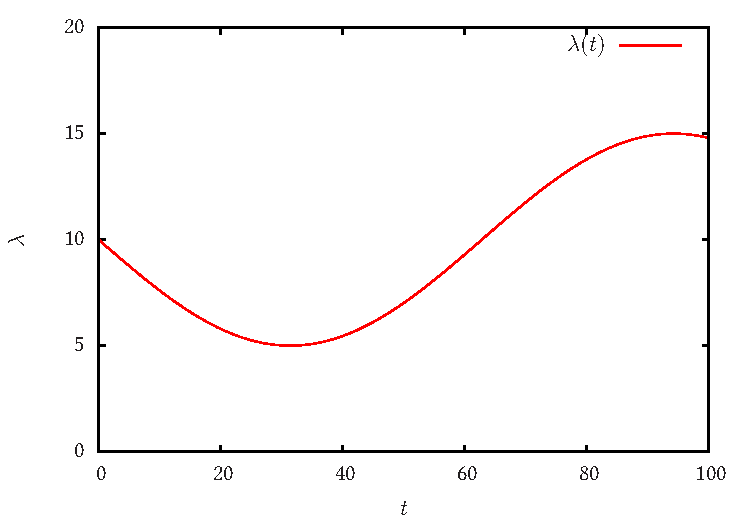
\includegraphics[width=0.5\textwidth]{images/prelim_sine_005}
  }
  \subfloat[$\alpha=0.01$]{
  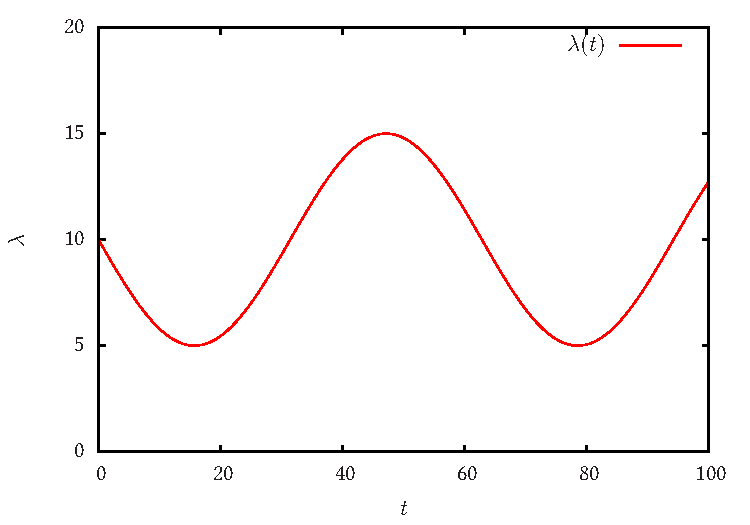
\includegraphics[width=0.5\textwidth]{images/prelim_sine_01}
  }\\
  \subfloat[$\alpha=0.015$]{
  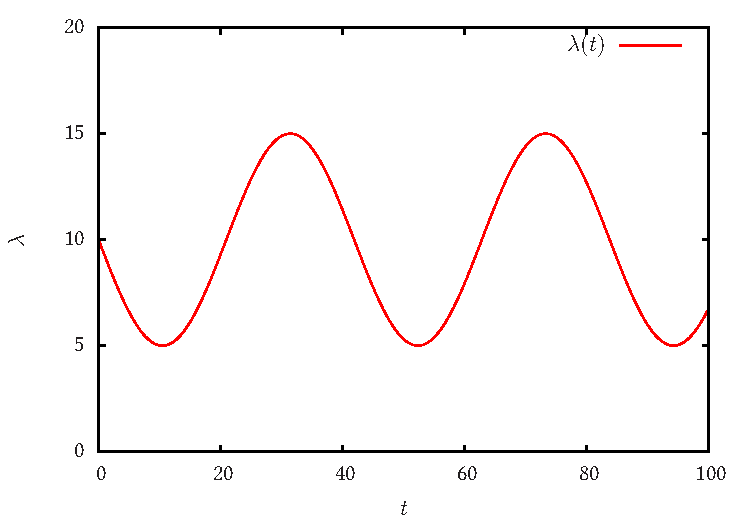
\includegraphics[width=0.5\textwidth]{images/prelim_sine_015}
  }
  \subfloat[$\alpha=0.03$]{
  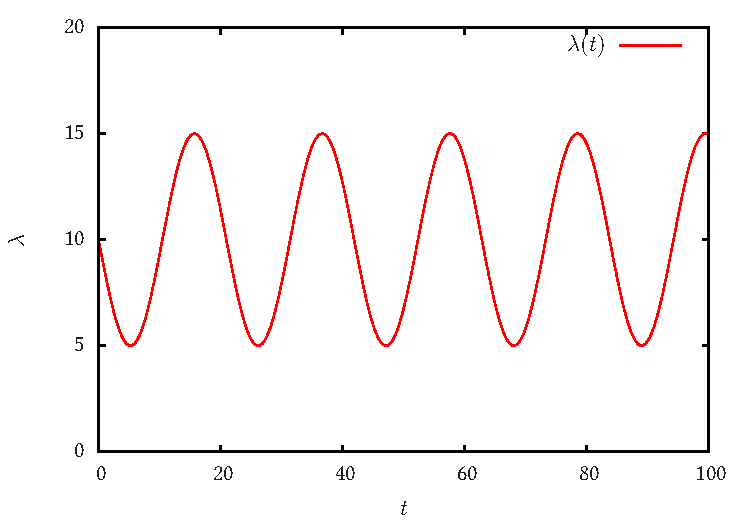
\includegraphics[width=0.5\textwidth]{images/prelim_sine_03}
  }\\
  \begin{center}
  \subfloat[$\alpha=0.06$]{
  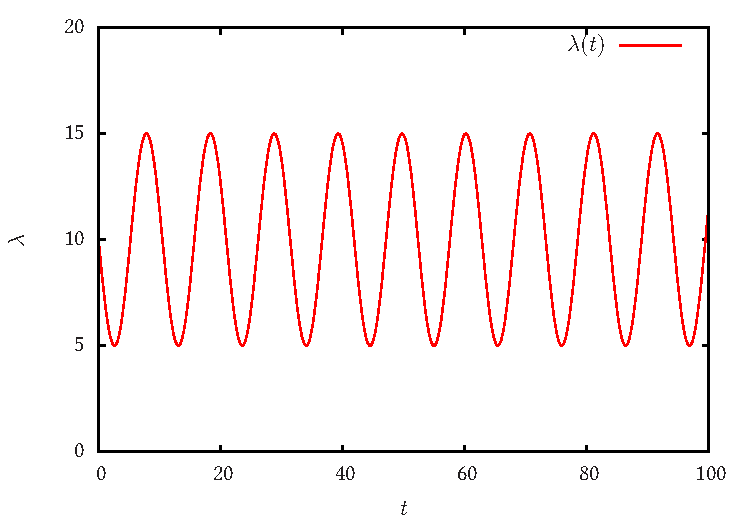
\includegraphics[width=0.5\textwidth]{images/prelim_sine_06}
  }
  \end{center}
  \caption{Functions used for preliminary experiments on sine functions, showing
  the different $\alpha$ values used. The generating function is $y=a-b\sin(\alpha t)$.}
  \label{fig:avals}
  \end{figure}
  The experiments are done in two stages. First, the optimum parameter set for
  each function that is being experimented on is found using model
  selection. Model selection involves withholding some of the data from the
  estimator by removing the event data from intervals uniformly distributed
  across the interval being estimated. Each function is estimated, and the value
  of the function in the regions where data was removed is compared to the value
  that would be expected had all the data been present. The score is calculated
  using the Poisson PDF, as in Equation \eqref{eq:normcalc}.

  The Gaussian estimator was set to sample the kernels at a resolution of 0.3
  time units, and the standard deviation of the kernels was varied. The baseline
  estimator was set to use 3 iterations of the IWLS estimator, and four other
  parameters were experimented on.
  \begin{description}
  \item[IWLS sub-intervals] 2, 4, 6, 8, 10
  \item[PDF threshold] 0.01 to 0.15 with a step of 0.01
  \item[Maximum extension] 5, 7, 9, 11, 13, 15, 17, 19, 20
  \item[Maximum breakpoints] As above
  \item[Gaussian standard deviation] 0.5 to 20 with a step of 0.5
  \end{description}
  The parameters were co-varied, meaning that each value for one
  of the parameter settings was tested with all possible values of the other
  parameters, for a total of 6115 possible combinations.

  Once the optimum parameter set has been found, the time delay for the pair of
  streams is estimated, using all the data that is available. From this we
  receive estimates of the time delay on which it is possible to perform
  statistical analysis. The mean, standard deviation and error for each estimate
  on each function is calculated, and from this we can examine the effectiveness
  of the estimates. The aim of the experiments is to compare the effectiveness
  of the time delay estimation with four method combinations: Gaussian area,
  Gaussian pdf, baseline area and baseline pdf. Two statistical tests were done
  on the experimental results. A paired $t$-test was used to check whether one
  method was better than another. For the second test, we took the error values
  for the two method combinations being compared, subtracted one from the other
  and performed a one-sample $t$-test on the resulting set of values. The full
  set of statistical test results can be seen in Appendix \ref{sec-11}.

  We assume that the distribution of the samples is Gaussian, but this may not be
  the case. However, full non-parametric testing is out of the scope of this project.
\subsection{Sine Functions}
\label{sec-8-1}

   The first experiment performed used stream data generated from functions of
   the form $y=a-b\sin(\alpha t)$. An increase in the value of $\alpha$
   increases the oscillation frequency of the sine wave, and a decrease reduces
   it. The value of $a$ indicates how much the wave is shifted along the
   $y$-axis, and $b$ determines the amplitude of the wave. The values of $a$ and
   $b$ were set to 10 and 5 respectively.
\subsubsection{Preliminary Experiments}
\label{sec-8-1-1}

    In the first set of experiments, we investigate the performance of the
    estimators on five values of $\alpha$: 0.05, 0.1, 0.15, 0.3 and 0.6. Figure
    \ref{fig:avals} gives an indication of what the functions look like. For
    each value of $\alpha$, 25 pairs of streams were independently generated, each
    with an interval of 100 time units and a time delay of 10 time steps between the
    two streams. 
    \begin{figure}[h!]
    \subfloat[Baseline area]{
    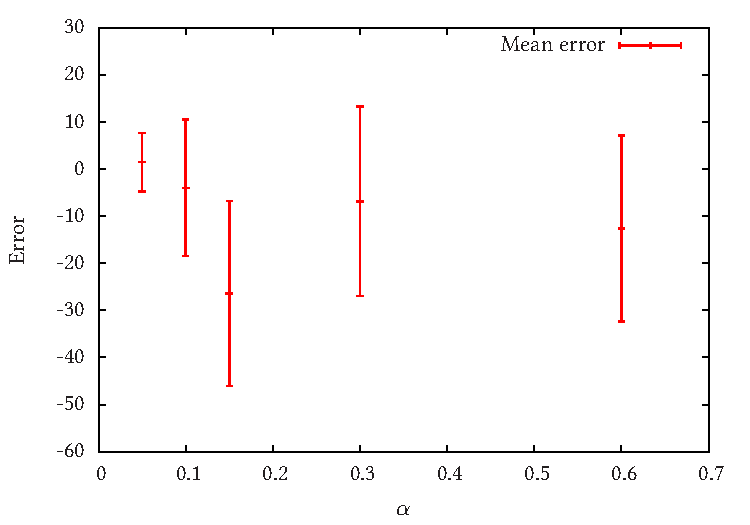
\includegraphics[width=0.5\textwidth]{images/base_area_prelim}
    }
    \subfloat[Baseline PDF]{
    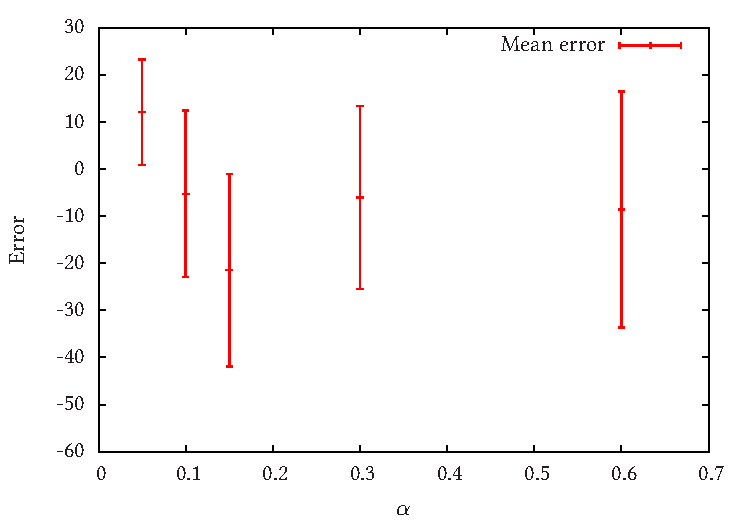
\includegraphics[width=0.5\textwidth]{images/base_pmf_prelim}
    }\\
    \subfloat[Gaussian area]{
    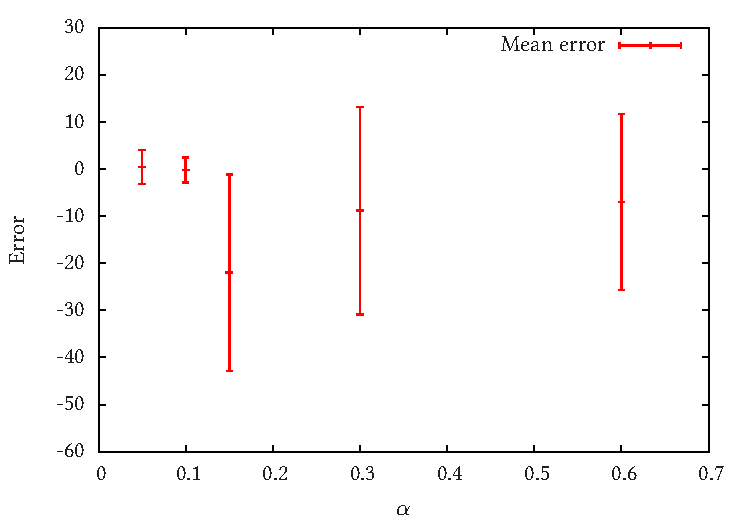
\includegraphics[width=0.5\textwidth]{images/gauss_area_prelim}
    }
    \subfloat[Gaussian PDF]{
    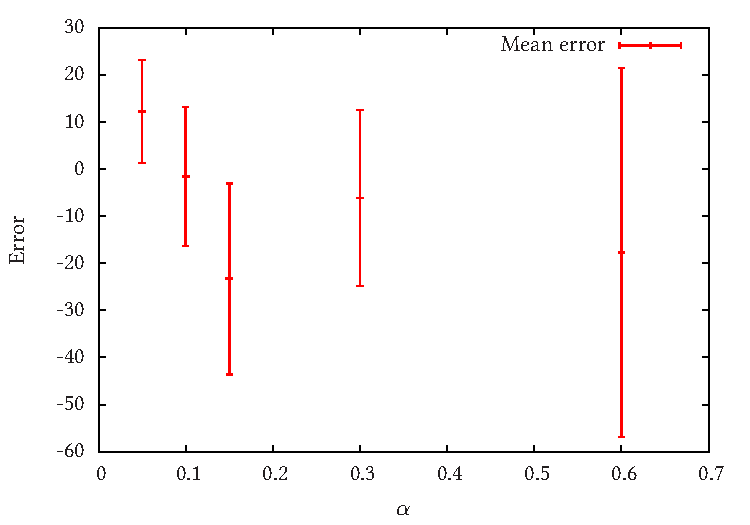
\includegraphics[width=0.5\textwidth]{images/gauss_pmf_prelim}
    }
    \caption{Mean error on the preliminary sine function experiments. Error bars show standard
    deviation of error. Performance appears to deteriorate when $\alpha>0.1$.}
    \label{fig:prelimerror}
    \end{figure}
    
    Figure \ref{fig:prelimerror} shows the error of the various estimator
    combination at each value of alpha. Performance appears optimal at low
    values of $\alpha$, with large standard deviation with $\alpha >$ 0.1. The area time
    delay estimator is significantly better than the PDF for both of the
    function estimators, with $p$-values of 0.00017 and 0.0000074 for the
    baseline and Gaussian method respectively at $\alpha=$ 0.05. The difference
    between the two function estimation methods was not significant, with
    $p$-values in excess of 0.4 for comparisons between the baseline and
    Gaussian estimators for the same time delay estimators at $\alpha=$
    0.05. Results from $\alpha>$ 0.005 show no statistical significance in the
    difference between the various estimators, so we cannot say whether the area
    estimator is always better.

\begin{table}[htb]
\caption{Experimental results for $\alpha=$ 0.05 for preliminary sine experiments. Actual time delay is 10. ($\mu\pm\sigma$)} \label{fig:pretab}
\begin{center}
\begin{tabular}{l|ll}
       &  Gaussian           &  Baseline           \\
\hline
 Area  &  10.39 $\pm$ 3.60   &  11.43 $\pm$ 6.18   \\
 PDF   &  22.20 $\pm$ 10.94  &  22.06 $\pm$ 11.20  \\
\end{tabular}
\end{center}
\end{table}
\subsubsection{Refined Experiments}
\label{sec-8-1-2}

    Although the previous set of experiments provide some indication as to the
    performance of the estimators, we investigated their effectiveness on a
    smaller range of $\alpha$ values. In this set of experiments, we used the
    same parameters, but generated a new set of functions for values of $\alpha$
    from 0.01 to 0.15, with a step of 0.01 between each successive set of stream
    pairs. 10 pairs of streams were generated for each $\alpha$ value. The time
    delay was set to 15 time units.
\begin{table}[htb]
\caption{Estimates for all method combinations at $\alpha=$ 0.07 for refined sine experiments. Actual time delay is 15. ($\mu\pm\sigma$)} \label{fig:reftab}
\begin{center}
\begin{tabular}{l|ll}
       &  Gaussian           &  Baseline           \\
\hline
 Area  &  15.99 $\pm$ 3.10   &  15.95 $\pm$ 4.51   \\
 PDF   &  16.53 $\pm$ 11.80  &  15.72 $\pm$ 14.06  \\
\end{tabular}
\end{center}
\end{table}

    The result of this second set of experiments uncovered an interesting
    pattern in the performance of the estimators. Figure \ref{fig:fineerror}
    shows the error for each combination of estimators for different values of
    $\alpha$. It is clear to see from the graphs that there is a window of
    optimum performance where $\alpha$ is between 0.04 and 0.1. We believe this
    may be as a result of the shape of the functions that are being
    estimated. As with the previous set of experiments, the area estimator again
    outperforms the PDF estimator, which is visible in the graphs and Table
    \ref{fig:reftab}. Within this window, the area method is significantly
    better than the PDF estimator in some cases, but this significance varies
    greatly with $\alpha$, and we therefore cannot conclude that there is a
    definite increase in accuracy using the area method. As before, the Gaussian
    and baseline methods were not significantly different.
    \begin{figure}[h!]
    \subfloat[Baseline area]{
    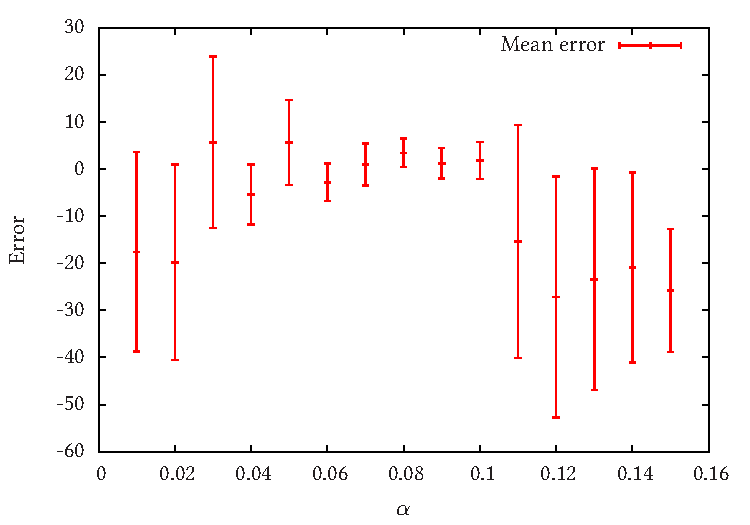
\includegraphics[width=0.5\textwidth]{images/baseline_area_fine}
    }
    \subfloat[Baseline PDF]{
    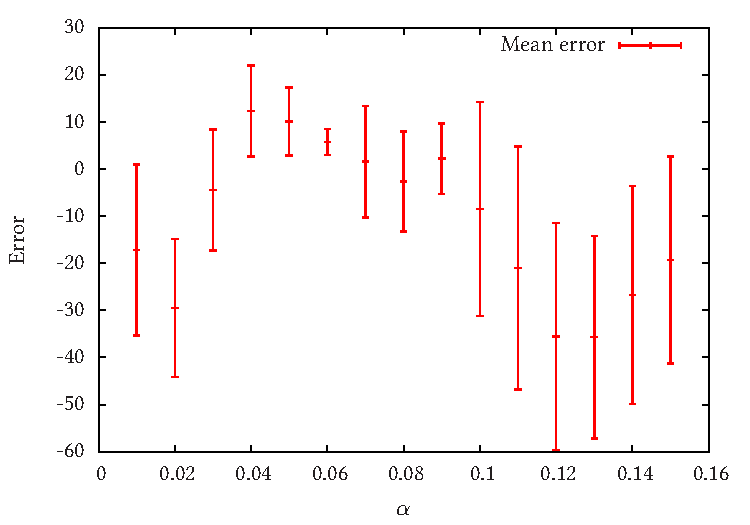
\includegraphics[width=0.5\textwidth]{images/baseline_pmf_fine}
    }\\
    \subfloat[Gaussian area]{
    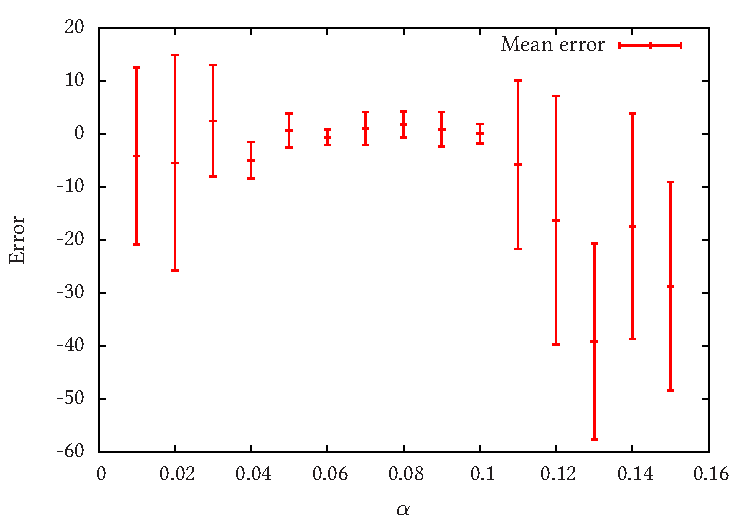
\includegraphics[width=0.5\textwidth]{images/gaussian_area_fine}
    }
    \subfloat[Gaussian PDF]{
    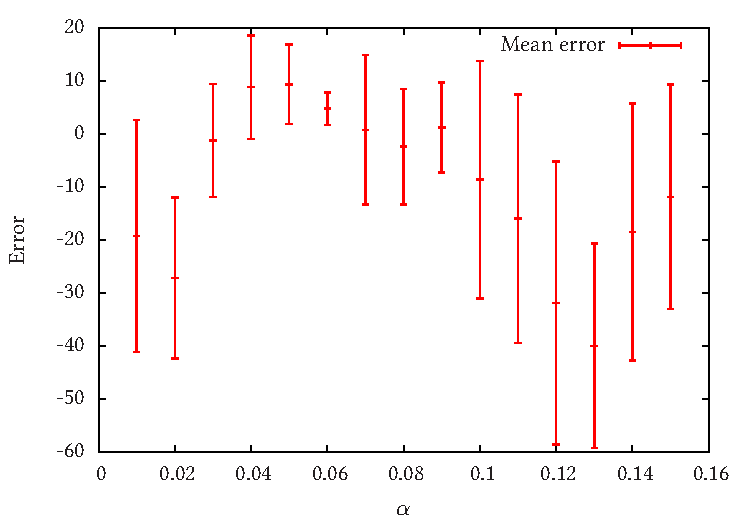
\includegraphics[width=0.5\textwidth]{images/gaussian_pmf_fine}
    }
    \caption{Error on the second set of sine function experiments. Error bars show
    standard deviation of error. Peak performance is in the window 0.04
    $\leq\alpha\leq$ 0.1}
    \label{fig:fineerror}
    \end{figure}
\subsection{Random Functions}
\label{sec-8-2}

   \begin{figure}
   \subfloat[$\alpha=0.4$]{
   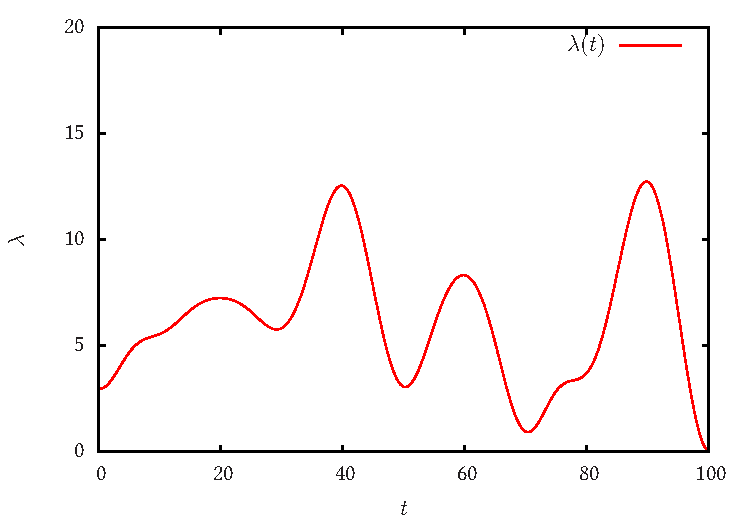
\includegraphics[width=0.5\textwidth]{images/randfunc_04}
   }
   \subfloat[$\alpha=0.8$]{
   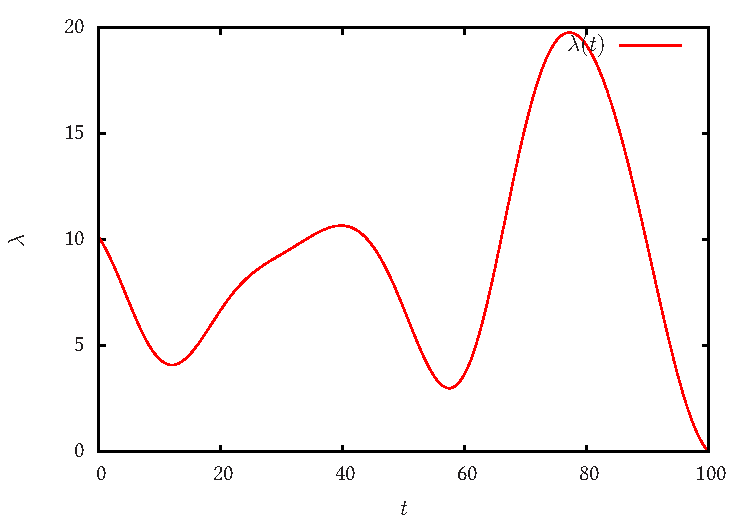
\includegraphics[width=0.5\textwidth]{images/randfunc_08}
   }\\
   \subfloat[$\alpha=1$]{
   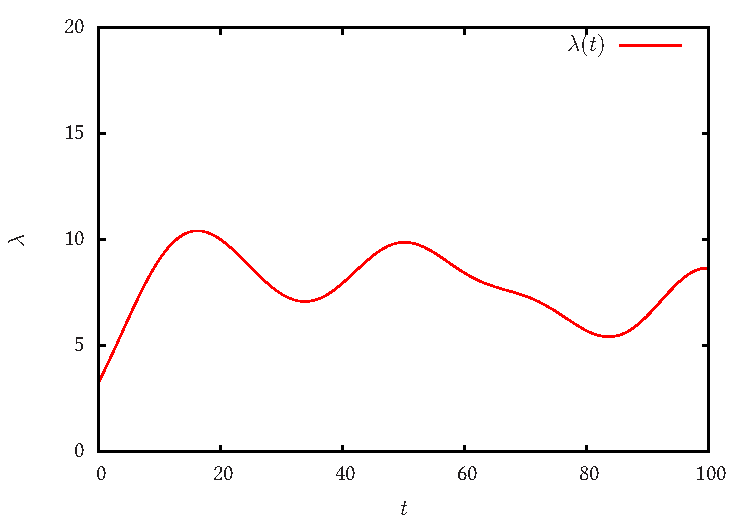
\includegraphics[width=0.5\textwidth]{images/randfunc_1}
   }
   \subfloat[$\alpha=2$]{
   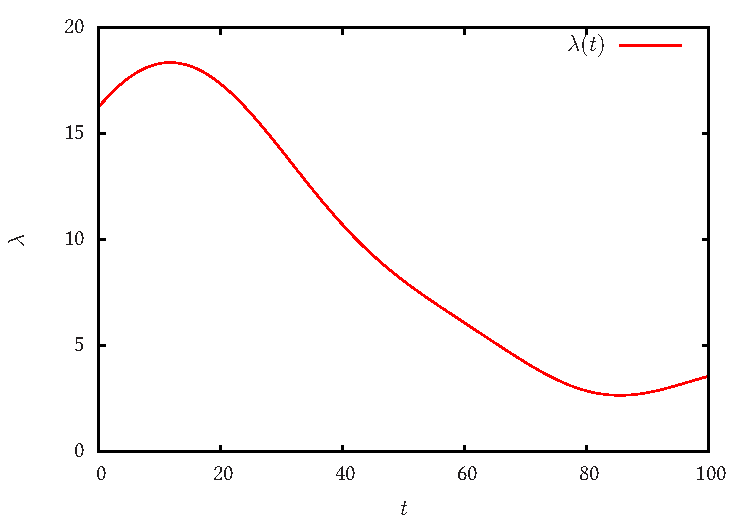
\includegraphics[width=0.5\textwidth]{images/randfunc_2}
   }\\
   \begin{center}
   \subfloat[$\alpha=3$]{
   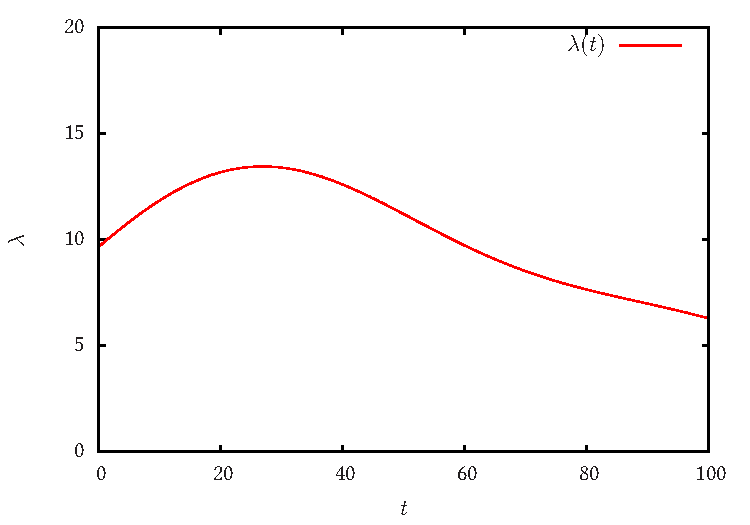
\includegraphics[width=0.5\textwidth]{images/randfunc_3}
   }
   \end{center}
   \caption{Examples of random functions generated by different
   values of $\alpha$. Oscillation of the functions decreases as $\alpha$ increases.}
   \label{fig:randex}
   \end{figure}
   The experiments on sine functions did not yield any definitive result as to
   which methods were more effective, and so we also performed a series of
   experiments using random functions rather than sine curves. Evaluating the
   performance of the estimators on these functions is important, since
   functions from real lensed objects will be very unlikely to follow a sine
   curve, instead fluctuating somewhat randomly. This set of experiments should
   also allow us to investigate the window of optimum performance from the
   previous experiment. In order to test a variety of different functions, we
   varied the $\alpha$ parameter in the equation $\sigma=\alpha\cdot\Delta t$,
   where $\sigma$ is the standard deviation of the Gaussians used to generate
   the random function. The weight of each Gaussian was set to 3, to produce a
   larger variation in the shape of functions. Figure \ref{fig:randex} shows
   some randomly selected examples.
\subsubsection{Preliminary Experiments}
\label{sec-8-2-1}

    For the preliminary experiment, we chose to use five different values of
    $\alpha$, 0.4, 0.8, 1, 2 and 3. While increasing the $\alpha$ parameter in the
    previous set of experiments would make the functions more difficult to estimate,
    in this case the opposite is true; larger values are easier to estimate, whereas
    smaller values are more difficult.
    
    For the preliminary experiments we set the value of $\Delta t$ to be 10,
    resulting in 11 Gaussians being spread uniformly across the 100 time unit
    interval. Given that $\alpha$ ranges from 0.4 to 3, the value of $\sigma$
    will be between 4 and 30 time units. Lower values of $\sigma$ result in each
    Gaussian being spread over a smaller interval, which in turn means that when
    the Gaussians are summed to construct the function it will have more
    variation than with large values. We generated 5 different functions for
    each value of $\alpha$, and from each of these generated 5 pairs of photon
    streams. In this preliminary experiment, we wish to see whether there is a
    clear point of deterioration, and whether there is any evidence of a window
    in which the methods are most effective.
    \begin{table}[htb]

    \centerline{
    \begin{tabular}{r|cccccc}
    $\alpha$  &  Baseline area        &  Baseline PDF         &  Gaussian area        &  Gaussian PDF         \\
    \hline
    0.4  &  2.884 $\pm$ 6.7225  &  -1.904 $\pm$ 10.82  &  1.62 $\pm$ 1.9959   &  0.132 $\pm$ 11.392  \\
    0.8  & 1.472 $\pm$ 4.6097  &   0.64 $\pm$ 4.566  &  0.424 $\pm$ 1.5155   &  0.644 $\pm$ 0.61407  \\
    1.0  & -7.784 $\pm$ 18.96   &  0.156 $\pm$ 8.9448  &  -1.4 $\pm$ 8.0519     &  -1.944 $\pm$ 9.1611  \\
    2.0  &   0.068 $\pm$ 0.64971   &  0.052 $\pm$ 3.0461  &  -0.068 $\pm$ 0.90184  &  -0.38 $\pm$ 4.2005   \\
    3.0  & 1.148 $\pm$ 0.99434   &  0.724 $\pm$ 5.9319  &  -0.156 $\pm$ 0.754  &  -0.824 $\pm$ 6.8956  \\
    \end{tabular}
    }
    \caption{Error values from the first set of random experiments. Error
    standard deviation is higher when $\alpha$ is 0.4 and 1.0. The area
    method appears to have lower standard deviations than the PDF method. ($\mu_{\text{err}}\pm\sigma$)}
    \label{tbl:frand}
    \end{table}
    The results from the experiment were very enlightening. Figure
    \ref{fig:randerror} shows the error of the estimators over all $\alpha$
    values. The estimators performed much more consistently, that the window in
    the sine experiments was due to the shape of the functions being
    estimated. The methods that we use seem to be ineffective on functions which
    have a symmetrical shape, which sine functions are. The estimators appear to
    be much more stable, with the mean error deviating relatively little from
    zero, in comparison to the large variation in the sine function experiments.

    While the performance of the estimators in terms of the mean error was
    better, the difference between method combinations is still not
    significant. The large error at $\alpha$ is 1 is due to very large errors
    occurring in estimates of two functions in that data set. This indicates
    that while on average the estimators perform well, on functions with certain
    characteristics there are large differences in the performance. Both time
    delay estimation methods have worse performance when $\alpha$ is 0.4, but
    the estimate from the area method is clearly less affected. Table
    \ref{tbl:frand} gives a better idea of the differences in the errors.

    \begin{figure}[h!]
    \subfloat[Baseline area]{
    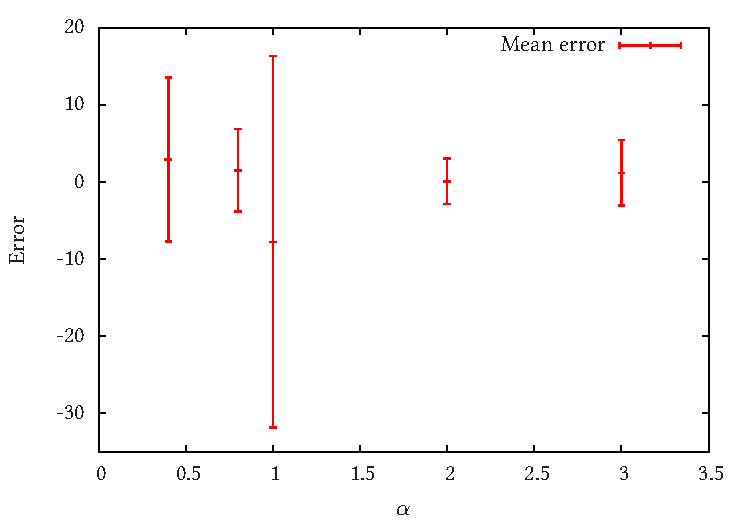
\includegraphics[width=0.5\textwidth]{images/baseline_area_random}
    }
    \subfloat[Baseline PDF]{
    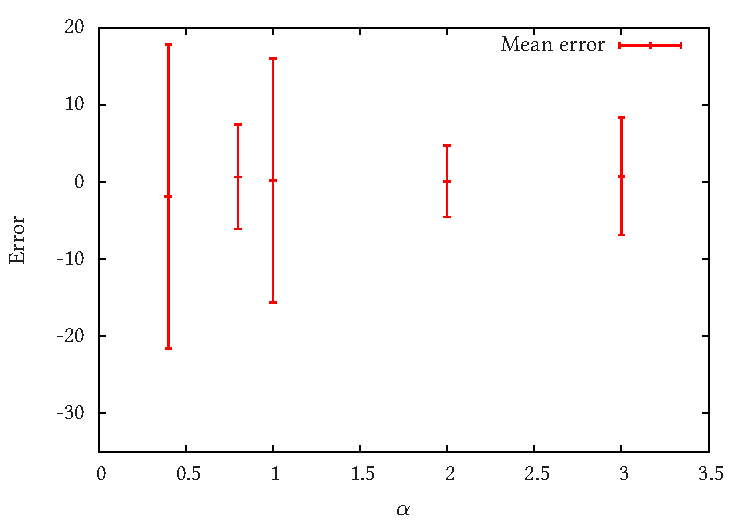
\includegraphics[width=0.5\textwidth]{images/baseline_pmf_random}
    }\\
    \subfloat[Gaussian area]{
    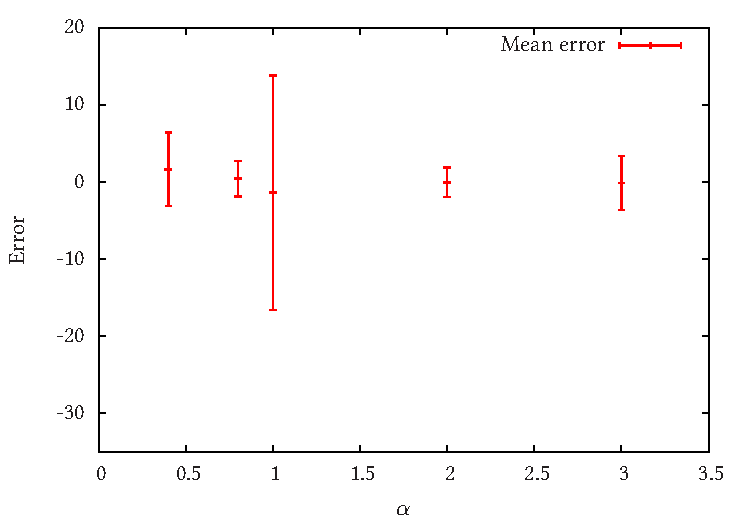
\includegraphics[width=0.5\textwidth]{images/gaussian_area_random}
    }
    \subfloat[Gaussian PDF]{
    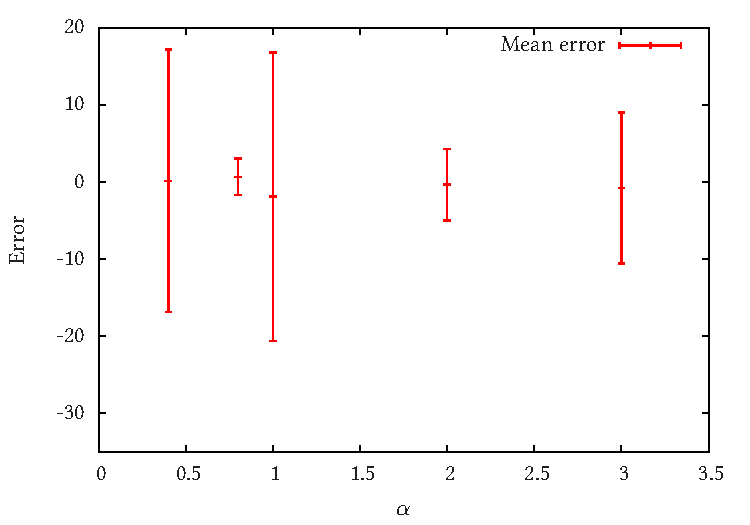
\includegraphics[width=0.5\textwidth]{images/gaussian_pmf_random}
    }
    \caption{Grand mean of error over 5 functions for each value of $\alpha$ for the preliminary random
    function experiments for each method combination.}
    \label{fig:randerror}
    \end{figure}
\subsubsection{Refined Experiments}
\label{sec-8-2-2}

    In order to investigate the estimator performance further, we performed an
    additional experiment on a finer set of data, varying $\alpha$ from 0.1 to
    1.5, with steps of 0.1. Going down to such a low value of $\alpha$ results
    in functions which have very large variations, with impulse-like peaks and
    troughs. The parameter ranges used were the same as in the previous
    experiment on random functions.

    This experiment confirms our observation from the previous experiment that the
    Gaussian area method combination is the one which should be used to get the best
    estimates with the smallest errors, which is clear to see in Figure
    \ref{fig:moreranderror}. Again, there was no pattern in the $p$-values that
    could be said to indicate that one method is significantly better than another,
    so we can not conclude with certainty that the Gaussian area method is indeed
    better than the others. However, this and previous experiments have shown that
    the size of the error from estimates with that combination is in the vast
    majority of cases smaller than that of other combinations. Errors appearing in
    combinations using the PDF method increase as values of $\alpha$ drop below 0.4,
    indicating that the method is more error-prone when functions have large
    variations. The PDF method in general has larger standard deviations on the
    error than the area method.
    \begin{figure}[h!]
    \subfloat[Baseline area]{
    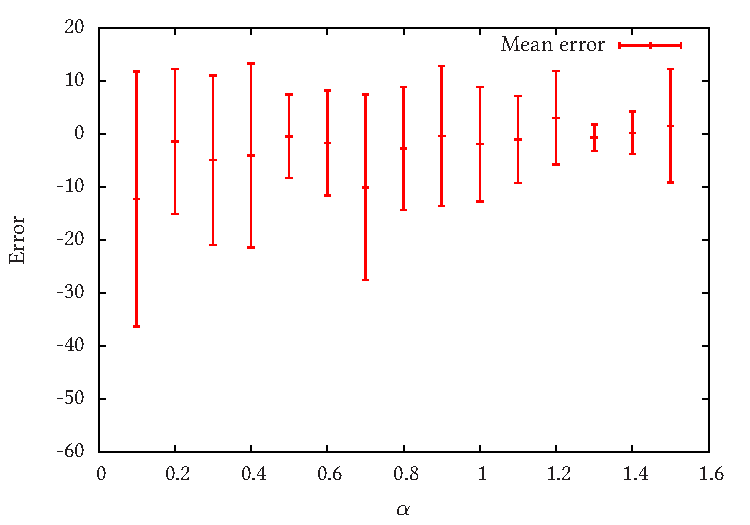
\includegraphics[width=0.5\textwidth]{images/baseline_area_morerand}
    }
    \subfloat[Baseline PDF]{
    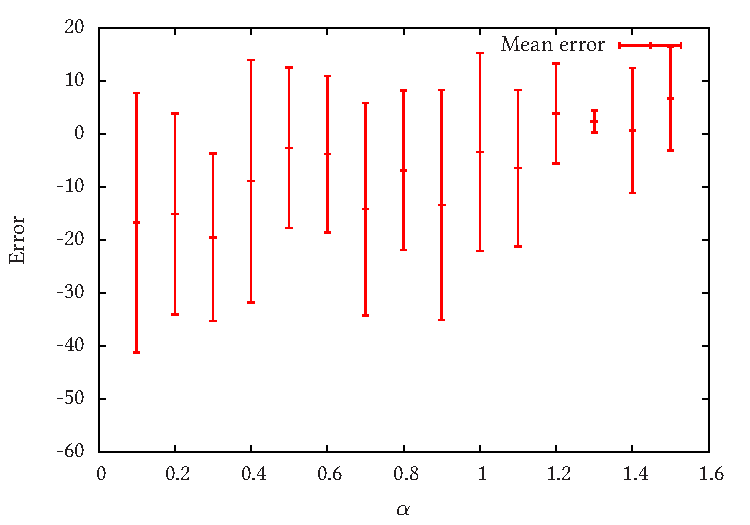
\includegraphics[width=0.5\textwidth]{images/baseline_pmf_morerand}
    }\\
    \subfloat[Gaussian area]{
    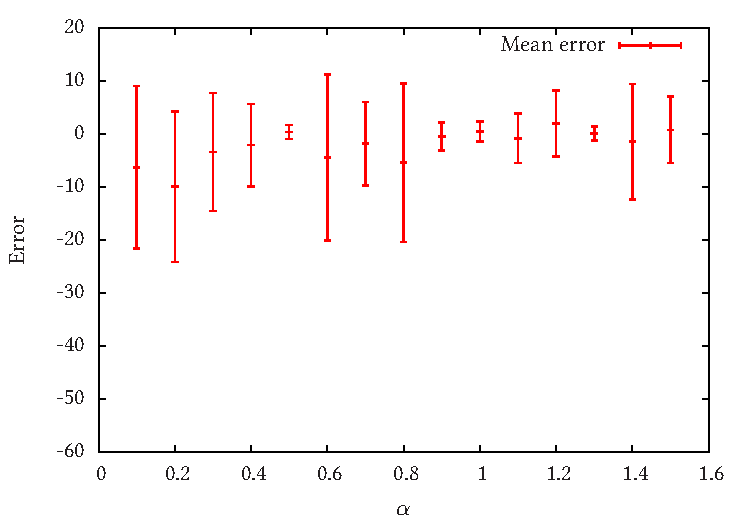
\includegraphics[width=0.5\textwidth]{images/gaussian_area_morerand}
    }
    \subfloat[Gaussian PDF]{
    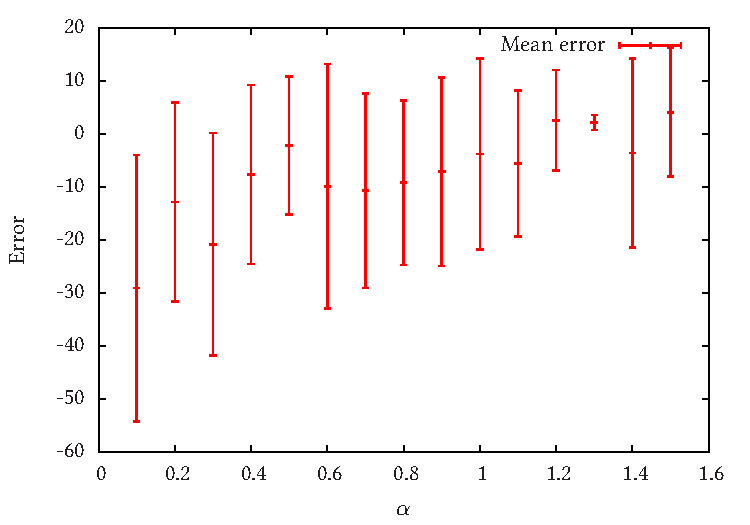
\includegraphics[width=0.5\textwidth]{images/gaussian_pmf_morerand}
    }
    \caption{Grand mean of error over 5 functions for each value of $\alpha$ for the second set of random
    function experiments for each method combination.}
    \label{fig:moreranderror}
    \end{figure}
\section{Conclusion}
\label{sec-9}

  In this report, we have presented our system for estimating the time delay in
  gravitationally lensed photon stream pairs. We showed two methods for
  estimating the characteristic function of the stream; the baseline method,
  which is built upon the iterative weighted least squares method described by
  Massey et al. \cite{massey1996estimating}, and the Gaussian kernel density
  estimation method, a simplified method similar to the one presented by
  Cuevas-Tello et al. \cite{cuevas2006accurate}. In addition, we presented two
  methods for time delay estimation, one using inter-function area, and another
  using probability density functions.

  We performed two sets of experiments to determine how well the estimators
  performed on sine functions and randomly generated functions, and found that
  while the difference is not significant, the Gaussian kernel density function
  estimation method combined with the inter-function area time delay estimation
  method appears to perform best in most cases. Appendix \ref{sec-11}
  contains a selection of the experimental results. From the experiments, we
  also learnt that the estimators may have worse performance on functions which
  have some sort of symmetry or repeating pattern, like sine functions.
  
  Having run the estimators with over 6000 different parameter combinations on
  multiple functions and with multiple stream pairs during experimentation, we
  are confident in the stability of the system. More formal checks of the
  correctness of the system are provided by unit tests for 62 functions which
  perform important tasks in the system.

  We have created a system that can complete all the tasks that we set out to
  implement. It can generate functions from predefined expressions and
  randomised Gaussians, and use these functions to generate photon streams using
  non-homogeneous Poisson processes. Our two function estimation methods provide
  good estimates of the characteristic function of the photon streams, and using
  these estimates, our time delay estimation methods produce time delay
  estimates close to the actual value in the majority of cases. We believe that
  the system is a good starting point for a larger system for automatic
  detection of potential gravitationally lensed objects. In the next section we
  provide some ideas for improvements which may make it a better foundation.
\subsection{Improvements and Future Work}
\label{sec-9-1}

   The first improvement is in the simulation of photon streams. Currently, the
   $\lambda$ parameter provided to the generator must be larger than the value
   of the function $\lambda(t),\,0\leq t\leq T$. This means that the maximum
   value of the function must be calculated before the program is run, or a
   value of $\lambda$ must be chosen such that the function is unlikely to
   exceed it. In most cases this does not pose a real issue, and large values of
   $\lambda$ can be chosen to no negative effect---the generation of data is
   still very fast. However, for ease of use of the system, implementing a
   method which does not require this parameter would be beneficial.Apart from
   the thinning method that we have used, there are many other methods of
   generating NHPPs \cite{pasupathy2011,lewis1976simulation} which could be
   implemented to improve this.

   There is also the potential for improvements to the baseline
   estimator. Currently, at each breakpoint only the midpoint is considered. A
   hierarchical search could improve the quality of estimates. Instead of
   considering only a single point, a search could be done along the line
   between the points to find the point at which the probability density
   function was maximised. If this was done for each breakpoint, then it should
   be possible to find a function which provides a better estimate than the
   current approach.

   Using a fast Gauss transform function in the kernel density estimator could
   improve its running time. In addition, exploring ways to mitigate the
   drop-off at the start and end of the interval would give more accurate
   estimates at these points.

   From our experiments, we discovered that the time delay estimators developed
   appear to perform worse on functions which have repeating patterns or are
   symmetrical in some way, such as the sine function. Adding confidence values
   to the time delay estimates would give more information to the user. Also,
   currently only the highest scoring value of $\Delta$ is reported. Reporting
   other peaks might provide information about periodicity.

   Although we have performed several experiments, we were unable to obtain real
   photon stream data on which to test our estimators. To find out whether our
   system would be useful in real applications, it should be applied to some
   real world data.

   As mentioned in the introduction, this system is intended to form a base for
   a system which can automatically identify potential gravitationally lensed
   objects. We believe that the current system provides a good foundation for
   such a system. However, given that its accuracy is limited, the ideal case is
   for this system to provide some sort of initial estimate, and then hand over
   to another system which is able to make more accurate estimates. We have
   identified three features that could be added as an extension to this system,
   or as separate systems:
\begin{enumerate}
\item Pull stream data from a database or some other form of storage
\item Compute likelihood of a pair of images coming from the same object based on
   estimates from our system
\item Keep track of which data has been processed and the confidence
   values of the estimates associated with that data
\end{enumerate}

   The combination of our system with a system or systems with these features would
   potentially create a system that could reasonably be applied to real-world problems.
\subsection{Individual Comments}
\label{sec-9-2}

   Although I have worked on several reasonably large projects during my time at
   university, this is the largest by far. Other projects of comparable size
   have been team projects, and as such I did not have to deal with the whole of
   the code base or management of the project. I believe that working alone on
   this project (other than weekly supervision meetings) has improved my
   abilities in many areas. 

   First and foremost, working on a project in a field which I have relatively
   little experience was quite a daunting task. Before starting I had some
   interest in machine learning, but my knowledge of problems and approaches to
   solving them was minimal. Developing the function estimators was particularly
   challenging, with literature on the subject being quite heavy on mathematics
   with which I was unfamiliar. I had to study the papers on which the function
   estimators are based for some time before I felt confident that I understood
   the important points. I have come to understand the techniques much better
   than I did initially, but there is still much to learn. Statistical testing
   was another challenging part of the project, requiring me to understand how
   various statistical techniques work, and which approaches are valid for what
   sort of data. Processing and analysing the results of the experiments was
   also new to me, but was a good learning experience which will be useful for
   any scientific projects I may encounter in the future.

   In addition to being in an unfamiliar field with new mathematical concepts, I
   also chose to write the project in C, a language which I had studied for only
   a short time before starting the project. Attempting to implement a complex
   system in a language which one is new to is difficult, and it took a few
   months before I was able to add new features and modify old code with the
   confidence and speed with which I can do so in other languages. C has a
   rather small set of standard libraries, and so I had to implement many
   features that are commonly available in the standard libraries of other
   languages. For more complex functionality, in order to save time I had to
   find libraries to use, and work out how to use a system with relatively
   sparse documentation and information available. I think that forcing myself
   into an uncomfortable situation in terms of unknown environments has paid
   off, as I am now confident in my C skills.

   During the course of the project, I had to make several decisions about the
   structure of the code, and make sweeping changes to the code base. One
   example is the point at which I made the switch from the use of pointer
   arrays to store estimate data to using structs. This required the
   modification of some of the fundamentals of the system and required great
   care to implement without introducing bugs. While in team environments it is
   possible to discuss structural changes and how to go about implementing a new
   feature, I had to rely on my own judgement to do both, which required a lot
   of time considering the benefits of one approach over another.

   I have learnt a lot from working on the project, and I hope to make good use
   of not only the technical knowledge, but also the experience of working on a
   large and challenging project in the future.

   \newpage
   \printbibliography
   \newpage

\begin{appendices}
\section{Usage}
\label{sec-10}
\subsection{Installation}
\label{sec-10-1}

   This installation guide is intended for users of Linux distributions,
   particularly those which are Ubuntu based. The program was tested on Linux
   Mint 13 and 14 on a 64 bit architecture, but should work on most Linux
   distributions. First, download the latest version of the program from
   \href{https://github.com/heuristicus/final-year-project/tags}{https://github.com/heuristicus/final-year-project/tags} and extract it with
   your favourite program. Alternatively, clone the current version of the
   repository with
   \begin{verbatimtab} 
   git clone [[https://github.com/heuristicus/final-year-project.git]]
   \end{verbatimtab}
   Before the program can be configured, we must install some libraries without
   which the program will not run. Download the latest muParser package from
   \href{http://sourceforge.net/projects/muparser/files/latest/download}{http://sourceforge.net/projects/muparser/files/latest/download} (must be
   $\geq$ v2.2.3). Then, run the following commands
   \begin{verbatimtab}
   unzip muparser_v_[your_version]
   cd muparser_v_[your_version]
   ./configure --prefix=/usr
   make && make install // may require sudo
   \end{verbatimtab}
   This will install muParser so that the header files it uses can be found in
   \texttt{/usr/include}. Your system must have the \texttt{g++} package
   installed for the \texttt{configure} command to complete, and you may also
   require the \texttt{autoconf} package. We must also install the GNU
   Scientific Library and the Check test framework. All the required packages
   can be installed with
   \begin{verbatimtab}
   apt-get install libgsl0-dev check g++ autoconf
   \end{verbatimtab}
   Once this is done run \texttt{./configure} followed by \texttt{make} in the
   program directory.
\subsection{General Usage}
\label{sec-10-2}

   The executable for the program can be found in the \texttt{src} directory,
   and is named \texttt{deltastream}. It can be run from the top level directory
   with
   \begin{verbatimtab}
   src/deltastream [OPTIONS]
   \end{verbatimtab}
   To find out what options are available, call the executable with the
   \texttt{-h} or \texttt{--help} options. We will detail some of the options
   below. All parameters which govern the behaviour of the system are defined in
   the parameter files, which have information about what the effect of each is.
\subsubsection{Parameter Files}
\label{sec-10-2-1}

    Some parameter files are provided with the program, but if for some reason
    they are deleted, then additional ones can be created using
    \begin{verbatimtab}
    deltastream -d paramfile.txt // default
    deltastream -d paramfile.txt -x a // experiment
    \end{verbatimtab}
\subsubsection{Generating Functions}
\label{sec-10-2-2}

    The \texttt{-g} switch is used to run all generation functions. Generating a
    random function can be done in one of two ways. Using
    \begin{verbatimtab}
    deltastream -g params.txt -r -c 1
    \end{verbatimtab}
    We can generate a file containing a Gaussian representation of a random
    function which we can use to generate streams. Changing the number passed
    to the \texttt{-c} switch changes the number of functions generated. To
    generate streams from the functions, we use
    \begin{verbatimtab}
    deltastream -g params.txt -f rand -n 2 -i random_function_0.dat
    \end{verbatimtab}
    This takes the data in the file \texttt{random\_function\_0.dat}, generated
    in the previous step, and generates two streams. Modifying the number passed
    to the \texttt{-n} option will generate different numbers of
    streams. Another way to generate random functions is with
    \begin{verbatimtab}
    deltastream -g params.txt -f rand -c 3 -n 2
    \end{verbatimtab}
    The \texttt{-c} switch defines how many functions should be generated. After
    the functions are generated, two streams are generated from each. If you
    wish to generate multiple different pairs of streams from the same function,
    use
    \begin{verbatimtab}
    deltastream -g params.txt -f rand -c 3 -n 2 -u
    \end{verbatimtab}
    The first function generated will be copied into multiple files, and streams
    will be generated from those copied files. The \texttt{-t} switch can be
    used to specify more or less verbose output. For example, passing a value of
    3 will output bin counts for the streams, and a file containing the sum of
    Gaussians which make up the random function.

    The generation of streams from expressions is rather simpler. The following
    two commands are equivalent.
    \begin{verbatimtab}
    deltastream -g params.txt -n 2
    deltastream -g params.txt -f mup -n 2
    \end{verbatimtab}
    The generator defaults to generating streams from the expression defined in
    the parameter file. Multiple pairs can be generated using the \texttt{-c} switch.
\subsubsection{Estimating Functions and Time Delay}
\label{sec-10-2-3}

    Estimates of functions are done using the \texttt{-e} switch. The most
    important parameters are defined in the parameter file. Once streams have
    been generated, we can estimate them using the baseline estimator
    \begin{verbatimtab}
    deltastream -e params.txt -a base -n 2
    \end{verbatimtab}
    If the streams were generated from a random function, the \texttt{-r} switch
    must be added to indicate this fact. Again, if there are multiple functions
    to estimate at once, use the \texttt{-c} switch to specify the number. The
    \texttt{-a} option has 5 possible arguments (\texttt{ols}, \texttt{iwls},
    \texttt{pc}, \texttt{base} and \texttt{gauss}), each of which use a
    different estimator to produce an estimate. Passing a value larger than 1 to
    the \texttt{-n} option will result in an estimate of the time delay. To
    estimate only the function, simply omit the switch.
\subsubsection{Plotting Output}
\label{sec-10-2-4}

    The \texttt{scripts/plot.sh} script can be used to plot various data which
    is output from the system. Calling it with the \texttt{-h} option will
    output information about what plots can be made. The script generates a
    \texttt{.tex} file using \texttt{gnuplot}, which it then processes into a
    \texttt{.pdf} and displays using \texttt{evince}. After doing a function
    estimate with the baseline estimator, the generating function can be plotted
    along with the bin data and estimate using 
    \begin{verbatimtab}
    scripts/plot.sh -f output random_function_0_sum.dat est_out.dat
    random_function_0_output_stream_0_bins.dat
    \end{verbatimtab}
\subsection{Running Experiments}
\label{sec-10-3}
\subsubsection{Creating Functions for Experimentation}
\label{sec-10-3-1}

    Using the \texttt{genfunc\_rand.sh} script found in the \texttt{scripts} directory, random
    functions can be generated, conforming to certain parameters. In this file,
    we specify the directory to which to output by modifying the
    \texttt{OUTPUT\_DIR} parameter. The \texttt{LAUNCHER\_LOC} parameter specifies the
    location of the \texttt{deltastream} executable used to run the program. The
    \texttt{PARAM\_FILE} parameter defines the location of the parameter file to use
    to generate the functions.

    Once these have been set, we specify the values to use to generate the
    function. The values in the the \texttt{AVALS} parameter define what values of
    $\alpha$ will be used to generate the functions. The \texttt{DIVISOR} parameter
    specifies what to divide the values in \texttt{AVALS} by when modifying the
    $\alpha$ parameter in the parameter file. This can be set to 1 to just use the
    values inside the array. The values in the \texttt{AVALS} array are also used to
    create directories, so the divisor is also used to prevent creation of
    directories such as \texttt{alpha\_0.3}. The \texttt{NFUNCS} parameter defines
    how many different functions to generate. \texttt{NPAIRS} defines the number of
    pairs of streams that will be generated from each function. Streams generated
    will be copies of the function. For example, when \texttt{NPAIRS} is set to 5, a
    function $f(a)$ is generated, along with two streams. Then, four more streams
    are generated from the same function $f(a)$. This allows for multiple trials on
    similar data. The \texttt{FPREF} and \texttt{APREF} define the text that is
    prepended to the directories. Setting \texttt{FPREF} to \texttt{function\_} and
    \texttt{APREF} to \texttt{alpha\_} will put each set of functions in a directory
    structure like \texttt{alpha\_1/function\_1}.
\subsubsection{Generating Model Selection Data}
\label{sec-10-3-2}

    Next, we use the \texttt{stutter\_batch.sh} script to generate streams with data
    removed in certain intervals to use for model selection. Here, we set the
    \texttt{INDIR} parameter to the directory which we set as the output directory
    in the previous script, and make sure to set the \texttt{AVALS}, \texttt{NFUNCS}
    and \texttt{NPAIRS} parameters to the same values. We must also define the
    \texttt{EXP\_PFILE} parameter, which tells the script where to look for the
    experimental parameters. In this file, we must set up which data should be
    removed. Modifying values in the \texttt{setup} section of the experiment
    parameter file will allow the choosing of various intervals. To generate a
    default experiment parameter file, use \texttt{deltastream -d [filename] -x
    a}. Once this is set up, we run the script, and it generates a new set of files
    in the same location as the original data which has data in some intervals
    removed, with names something like \texttt{random\_function\_0\_output\_stream\_0\_stuttered.dat}.
\subsubsection{Experiment Parameter Setup}
\label{sec-10-3-3}

    Now, we set up the experiments that we wish to perform on the data. In the
    experiment parameter file, there are various options which control how the
    experiments are run. The most important is the \texttt{experiment\_names}
    parameter, which defines the names of the experiments that you wish to run. Once
    the names are set, we must define four parameters that are used to run the experiment.
    \small
    \begin{verbatimtab}
    experiment_names exp_1,exp_2 // Name the experiments
    // These parameters will be varied during the experiments
    exp_1_params base_max_breakpoints,base_max_extension
    exp_2_params gauss_est_stdev
    test_exp_1 yes // We want to experiment on this
    test_exp_2 no // This will not be experimented on
    // Set the estimator to use for the experiment
    exp_1_estimator base 
    ext_2_estimator gauss
    // Estimate the function or the time delay
    exp_1_type function
    exp_2_type delay

    // Set the parameter values for experiments
    base_max_extension 3,6,...,11
    base_max_breakpoints 4,5,...,10
    gauss_est_stdev 1,2,3,4

    // This is important! Set the time delay between streams
    // Used later to analyse the results
    timedelta 0,15
    \end{verbatimtab}
    \normalsize

    When setting the parameter values, \texttt{...} can be used to specify a
    range. In the example, the \texttt{base\_max\_extension} parameters would be 3,
    6, 9 and 11. The \texttt{timedelta} parameter is important as well---it provides
    the program with the actual value of the time delay between streams, which is
    used to determine the score of certain parameter settings. Information about the
    parameters used to generate streams can be found in the output directories in
    the \texttt{gen\_params.txt} file.
\subsubsection{Running Model Selection}
\label{sec-10-3-4}

    Once the parameters are set up, we run model selection on the generated streams
    using the \texttt{runexp\_batch.sh} script. Here we again set the various
    parameters needed, and specify a new output directory into which the experiment
    data is output. Depending on the number of experiments being run, the data can
    take up a lot of space (on the order of gigabytes), so choose a disk with plenty
    of free space. It is also a good idea to run a small subset of the experiments
    before running them all, just to make sure that you are outputting to the
    correct directory---\textbf{data in the output directories from previous
    experiments is overwritten}. Once you are sure that everything is good to go,
    run the script. Time taken depends on the number of parameter combinations and
    number of functions you are running the experiments on. A reasonably large set
    of data (approximately 151,000 experiments) took approximately two hours on an
    Intel i5 processor.
\subsubsection{Time Delay Calculation}
\label{sec-10-3-5}

    Once the experiments have completed, we use the best parameter settings from the
    model selection stage to run time delay estimators on the data again, this time
    with all data available to the estimators. First, we use the
    \texttt{get\_goodness.sh} script to extract the experiment numbers of the
    highest scoring parameter settings. Inside the \texttt{runtd\_exp.sh} file, we
    modify the relevant parameters, setting the parameter files to read from, the
    directory from which to read the parameter data---the directory set as the
    output directory for the model selection, the location in which the files output
    from the \texttt{get\_goodness.sh} script, and the place where we wish to put
    the files produced by this stage of the process. When the script is run, it
    performs a time delay estimation on the streams with the best parameters for
    each function and $\alpha$ value. Inside each directory, a file
    \texttt{results.txt} is produced, which contains the some data about the
    performance of the estimators with that combination of methods on the given
    $\alpha$ value for that function. In the next step, we extract this data into a
    more usable form.
\subsubsection{Extracting Result Data}
\label{sec-10-3-6}

    In the \texttt{extract\_results.sh} script, we set up the parameters so that
    \texttt{INDIR} is set to read from the top level of the time delay results
    directory, and \texttt{OUTDIR} is set to the location to which we wish to output
    the aggregated results. There are three different flags that can be set to
    produce data in different forms for processing. The \texttt{TT} flag makes the
    script output error data in a form in which it can be processed by other scripts
    to run t-tests. The \texttt{DV} flag outputs data which can be used to calculate
    the mean value of the time delay estimate across all functions. Usually, the
    means are calculated on a per-function basis, but setting this flag outputs data
    in a form which groups data from all the functions for one value of $\alpha$
    into one set which can then be easily processed as a single set of
    estimates. The \texttt{EV} flag does a similar thing to the \texttt{DV} flag,
    but for error data. The error values are grouped by $\alpha$ value, and the
    resulting files can be used to find the aggregate error for each value of
    $\alpha$ for a specific method combination. Running the
    \texttt{extract\_results.sh} script will output the data. Next, we will explain
    how to process the resulting files.
\subsubsection{Processing Result Data}
\label{sec-10-3-7}

    Inside the results directory, the top level contains files which detail the mean
    estimate, standard deviation and mean error for each function for each value of
    $\alpha$. The \texttt{results} directory contains directories with files which
    are used to produce different data. The \texttt{data} directory contains copies
    of all results files, with the filenames showing what experiment the file was
    taken from.

    \paragraph{T-tests}

    To create data for t-tests, we use the files in the \texttt{alpha\_errors}
    directory. With this data we will be able to compare the errors of one
    combination of method to another. The \texttt{ttest\_columnate\_agg.sh} and
    \texttt{ttest\_columnate\_individual.sh} scripts are used to process the data
    further into files readable by the \texttt{ttest.m} script. The first script
    groups data so that when the t-tests are run, results from all functions for one
    value of $\alpha$ for one method are compared to the same set of functions for
    the same value of $\alpha$, but with a different method combination. The second
    script processes data so that results for individual functions are compared,
    rather than an aggregate set of data. T-test data will be output to a directory
    \texttt{ttest} in the directory specified in the script. In each file, there
    will be columns of data used for the t-test, as well as some information about
    where the data was taken from.

    Using the \texttt{ttest.m} script, we can run t-tests on the data. The script
    was written using GNU Octave, but should also be compatible with
    Matlab. The \texttt{read\_start\_x}, \texttt{read\_start\_y},
    \texttt{read\_end\_x} and \texttt{read\_end\_y} must be modified to match the
    data before the script is run. These values specify the range used by the
    \texttt{dlmread} command to parse in data from the files. In the case of 4
    columns with 25 lines each, the values are set to \small
    \begin{verbatimtab}
    read_start_x=0
    read_start_y=0
    read_end_x=24
    read_end_y=3
    \end{verbatimtab}
    \normalsize
    When run, the script produces a set of t-tests from the data. The
    \texttt{paired\_tests} matrix contains the results of two-tailed paired t-tests
    on the data, and the \texttt{single\_sample} matrix contains the results of
    single sample t-tests on the error values calculated by subtracting one set of
    data from the other. The comparisons array indicates which columns were compared
    to produce each column of the matrix. In general, 1 refers to the baseline area
    method, 2 to the baseline PDF method, 3 to the Gaussian area method, and 4 to
    the Gaussian PDF method.

    \paragraph{Mean and Standard Deviation of Estimates} Using the \texttt{multifunc\_mean.sh} script, the mean
    and standard deviation of estimates from different combinations of methods can
    be generated. Setting the \texttt{INDIR} variable to point to the
    \texttt{results/estimates} directory will perform the computations using a short
    Octave script, and output the results to a file, which will additionally contain
    tables for use in Emacs' \texttt{org-mode}. Tables \ref{tbl:sine1} and
    \ref{tbl:sine2} are examples of these tables converted into \LaTeX using the
    export functionality built into \texttt{org-mode}.

    \paragraph{Error of Estimates}
    Being able to display the error of combinations of methods, such as the graphs
    in Figures \ref{fig:prelimerror} and \ref{fig:fineerror} is also useful, and
    data to do this can be produced by the \texttt{multifunc\_errmean.sh}
    script. The script will produce files for each combination of methods, which can
    then be plotted with a program such as gnuplot. One way to plot the data using
    gnuplot is
    \small
    \begin{verbatimtab}
    plot "baseline_area_err.txt" using 1:2:3 with errorbars
    \end{verbatimtab}
    \normalsize
\subsection{CD Directory structure}
\label{sec-10-4}

   The \texttt{code} directory contains the scripts, tests, source code and
   documents for the project. The \texttt{experiments} directory contains
   experimental data and results. Data is contained within zip files in the
   subdirectories. Files with the \texttt{time\_delay} suffix contain the
   results of the time delay estimation after model selection was performed. The
   \texttt{streams} suffix contains the functions that were estimated, and the
   \texttt{results} suffix contains some processed results.
\section{Experimental Data}
\label{sec-11}

  In this appendix we present the full set of experimental data. BA=baseline area,
  GA=Gaussian area, BP=baseline PDF, GP=Gaussian PDF. BA/GA indicates a test
  comparing the Gaussian area method against the baseline area method.

  \begin{table}[htb]

  \begin{center}
  \begin{tabular}{r|llll}
  $\alpha$  &  Baseline area       &  Gaussian area        &  Baseline PDF         &  Gaussian PDF         \\
  \hline
  0.05  &  11.432 $\pm$ 6.18   &  10.388 $\pm$ 3.60    &  22.064 $\pm$ 11.20   &  22.20 $\pm$ 10.94    \\
  0.10  &  6.008 $\pm$ 14.46   &  9.76 $\pm$ 2.67      &  4.712 $\pm$ 17.68    &  8.42 $\pm$ 14.73     \\
  0.15  &  -16.44 $\pm$ 19.62  &  -12.024 $\pm$ 20.85  &  -11.472 $\pm$ 20.41  &  -13.308 $\pm$ 20.26  \\
  0.30  &  3.152 $\pm$ 20.09   &  1.14 $\pm$ 22.01     &  3.94 $\pm$ 19.40     &  3.84 $\pm$ 18.67     \\
  0.60  &  -2.62 $\pm$ 19.71   &  3.00 $\pm$ 18.65     &  1.404 $\pm$ 25.02    &  -7.744 $\pm$ 39.14   \\
  \end{tabular}
  \end{center} \caption{Table of mean estimate and standard deviation for
  combinations of methods on the first set of sine experiments ($\mu\pm\sigma,\,
  n=$ 25). The actual time delay is 10.} \label{tbl:sine1}\end{table}


  \begin{table}[htb]

  \begin{center}
  \centerline{
  \begin{tabular}{r|cccccc}
  $\alpha$  &    BA/GA  &       BA/BP  &       BA/GP  &              GA/BP  &               GA/GP  &    BP/GP  \\
  \hline
  0.05  &  0.47815  &  0.00017369  &  0.00011531  &  \num{0.000012894}  &  \num{0.0000073895}  &  0.96623  \\
  0.10  &  0.21721  &     0.78218  &     0.56963  &            0.17294  &             0.66295  &  0.43371  \\
  0.15  &  0.45352  &     0.39424  &     0.58888  &            0.92654  &             0.82960  &  0.75580  \\
  0.30  &  0.74226  &     0.89066  &     0.90272  &            0.64223  &             0.64879  &  0.98556  \\
  0.60  &  0.31540  &     0.53891  &     0.56946  &            0.80325  &             0.23073  &  0.33954  \\
  \end{tabular}
  }
  \end{center}
  \caption{Table of paired t-test $p$-values for preliminary sine experiments} \end{table}


  \begin{table}[htb]

  \begin{center}
  \centerline{
  \begin{tabular}{r|cccccc}
  $\alpha$  &    BA/GA  &              BA/BP  &              BA/GP  &               GA/BP  &               GA/GP  &    BP/GP  \\
  \hline
  0.05  &  0.40134  &  \num{0.000034334}  &  \num{0.000027901}  &  \num{0.0000037237}  &  \num{0.0000045120}  &  0.87340  \\
  0.10  &  0.19016  &            0.77691  &            0.58516  &             0.16046  &             0.65594  &  0.35306  \\
  0.15  &  0.44337  &            0.39762  &            0.54968  &             0.92600  &             0.84756  &  0.72240  \\
  0.30  &  0.77304  &            0.90010  &            0.89556  &             0.60185  &             0.54686  &  0.98399  \\
  0.60  &  0.25471  &            0.49996  &            0.56251  &             0.75755  &             0.22830  &  0.27032  \\
  \end{tabular}
  }
  \end{center} \caption{Table of $p$-values for preliminary sine experiments for
  one sample t-test performed on error values} \end{table}


  \begin{table}[htb]

  \begin{center}
  \centerline{
  \begin{tabular}{r|llll}
  $\alpha$  &  Baseline area       &  Gaussian area       &  Baseline PDF        &  Gaussian PDF        \\
  \hline
  0.01  &  -2.60 $\pm$ 21.17   &  10.81 $\pm$ 16.69   &  -2.21 $\pm$ 18.15   &  -4.32 $\pm$ 21.91   \\
  0.02  &  -4.80 $\pm$ 20.77   &  9.49 $\pm$ 20.36    &  -14.51 $\pm$ 14.65  &  -12.22 $\pm$ 15.20  \\
  0.03  &  20.67 $\pm$ 18.17   &  17.41 $\pm$ 10.52   &  10.49 $\pm$ 12.84   &  13.72 $\pm$ 10.65   \\
  0.04  &  9.58 $\pm$ 6.36     &  9.97 $\pm$ 3.44     &  27.3 $\pm$ 9.61     &  23.75 $\pm$ 9.77    \\
  0.05  &  20.58 $\pm$ 9.03    &  15.61 $\pm$ 3.21    &  25.06 $\pm$ 7.20    &  24.30 $\pm$ 7.48    \\
  0.06  &  12.17 $\pm$ 3.97    &  14.30 $\pm$ 1.48    &  20.72 $\pm$ 2.74    &  19.71 $\pm$ 3.09    \\
  0.07  &  15.95 $\pm$ 4.51    &  15.99 $\pm$ 3.10    &  16.53 $\pm$ 11.80   &  15.72 $\pm$ 14.06   \\
  0.08  &  18.42 $\pm$ 3.03    &  16.70 $\pm$ 2.46    &  12.35 $\pm$ 10.60   &  12.52 $\pm$ 10.93   \\
  0.09  &  16.19 $\pm$ 3.24    &  15.83 $\pm$ 3.25    &  17.16 $\pm$ 7.50    &  16.17 $\pm$ 8.51    \\
  0.10  &  16.79 $\pm$ 3.95    &  15.01 $\pm$ 1.82    &  6.48 $\pm$ 22.69    &  6.31 $\pm$ 22.38    \\
  0.11  &  -0.36 $\pm$ 24.73   &  9.13 $\pm$ 15.92    &  -6.03 $\pm$ 25.82   &  -1.06 $\pm$ 23.42   \\
  0.12  &  -12.19 $\pm$ 25.52  &  -1.36 $\pm$ 23.43   &  -20.62 $\pm$ 24.16  &  -16.97 $\pm$ 26.66  \\
  0.13  &  -8.42 $\pm$ 23.48   &  -24.21 $\pm$ 18.47  &  -20.71 $\pm$ 21.45  &  -25.04 $\pm$ 19.28  \\
  0.14  &  -5.96 $\pm$ 20.16   &  -2.49 $\pm$ 21.27   &  -11.75 $\pm$ 23.12  &  -3.53 $\pm$ 24.27   \\
  0.15  &  -10.83 $\pm$ 13.07  &  -13.80 $\pm$ 19.64  &  -4.36 $\pm$ 21.96   &  3.07 $\pm$ 21.17    \\
  \end{tabular}
  }
  \end{center} \caption{Table of mean estimate and standard deviation for
  combinations of methods on the second set of sine experiments
  ($\mu\pm\sigma,\,n=$ 10). The actual time delay is 15.}
  \label{tbl:sine2}\end{table}


  \begin{table}[htb]

  \begin{center}
  \centerline{
  \begin{tabular}{r|cccccc}
  $\alpha$  &      BA/GA  &             BA/BP  &       BA/GP  &               GA/BP  &       GA/GP  &      BP/GP  \\
  \hline
  0.01  &    0.15295  &           0.96699  &     0.86740  &             0.13054  &     0.11670  &    0.82642  \\
  0.02  &   0.157811  &          0.266797  &    0.398533  &            0.010178  &    0.019558  &   0.748621  \\
  0.03  &    0.64686  &           0.18670  &     0.33527  &             0.22703  &     0.46908  &    0.56859  \\
  0.04  &    0.87326  &         0.0002154  &   0.0018482  &   \num{0.000075319}  &  0.00085570  &    0.44706  \\
  0.05  &  0.1371851  &         0.2597158  &   0.3539836  &           0.0020559  &   0.0049413  &  0.8286646  \\
  0.06  &    0.14919  &  \num{0.00004719}  &  0.00027971  &  \num{0.0000078065}  &  0.00016456  &    0.47247  \\
  0.07  &    0.98273  &           0.89192  &     0.96325  &             0.89579  &     0.95576  &    0.89615  \\
  0.08  &    0.20268  &           0.11576  &     0.13599  &             0.24583  &     0.27772  &    0.97364  \\
  0.09  &    0.81655  &           0.72573  &     0.99482  &             0.63121  &     0.91209  &    0.79640  \\
  0.10  &    0.23567  &           0.19600  &     0.18339  &             0.27572  &     0.26019  &    0.98741  \\
  0.11  &    0.34587  &           0.63994  &     0.95152  &             0.15109  &     0.29466  &    0.67393  \\
  0.12  &    0.36082  &           0.48103  &     0.70215  &             0.10321  &     0.20355  &    0.76434  \\
  0.13  &    0.13020  &           0.26141  &     0.11813  &             0.71497  &     0.92673  &    0.65779  \\
  0.14  &    0.72652  &           0.57817  &     0.81986  &             0.38812  &     0.92404  &    0.47133  \\
  0.15  &   0.710077  &          0.457267  &    0.110994  &            0.349136  &    0.096720  &   0.474311  \\
  \end{tabular}
  }
  \end{center} \caption{Table of paired t-test $p$-values for second set of sine
  experiments.} \end{table}


  \begin{table}[htb]

  \begin{center}
  \centerline{
  \begin{tabular}{r|cccccc}
  $\alpha$  &     BA/GA  &              BA/BP  &       BA/GP  &              GA/BP  &       GA/GP  &     BP/GP  \\
  \hline
  0.01  &  0.238363  &           0.963181  &    0.834164  &           0.109943  &    0.083662  &  0.718245  \\
  0.02  &  0.012781  &           0.337071  &    0.318196  &           0.020011  &    0.011247  &  0.693379  \\
  0.03  &   0.70689  &            0.28411  &     0.42725  &            0.17888  &     0.27976  &   0.46476  \\
  0.04  &   0.85129  &  \num{0.000056159}  &   0.0016052  &  \num{0.000071618}  &  0.00051425  &   0.11740  \\
  0.05  &   0.13016  &            0.29164  &     0.38843  &         0.00076639  &   0.0017663  &   0.20065  \\
  0.06  &   0.12141  &         0.00027185  &  0.00054176  &  \num{0.000034371}  &  0.00034019  &  0.058177  \\
  0.07  &   0.96101  &            0.89812  &     0.96606  &            0.89112  &     0.95491  &   0.65016  \\
  0.08  &  0.093847  &           0.128048  &    0.147634  &           0.223662  &    0.252733  &  0.634744  \\
  0.09  &   0.71169  &            0.73272  &     0.99485  &            0.66951  &     0.91808  &   0.36155  \\
  0.10  &   0.28488  &            0.22685  &     0.21387  &            0.29118  &     0.27635  &   0.66831  \\
  0.11  &   0.23385  &            0.66956  &     0.95495  &            0.10105  &     0.18555  &   0.61964  \\
  0.12  &   0.42867  &            0.60176  &     0.75116  &            0.11260  &     0.20142  &   0.67466  \\
  0.13  &   0.16087  &            0.33354  &     0.14625  &            0.48521  &     0.91090  &   0.37568  \\
  0.14  &   0.74527  &            0.64935  &     0.84987  &            0.33823  &     0.91812  &   0.15872  \\
  0.15  &   0.74025  &            0.52892  &     0.17196  &            0.40520  &     0.18736  &   0.39848  \\
  \end{tabular}
  }
  \end{center} \caption{Table of $p$-values for second set of sine experiments for
  one-sample t-test performed on error values} \end{table}



  \begin{table}[htb]

  \begin{center}
  \centerline{
  \begin{tabular}{r|cccccc}
  $\alpha$  &  Baseline area        &  Baseline PDF         &  Gaussian area        &  Gaussian PDF         \\
  \hline
  0.4  &  17.884 $\pm$ 10.465  &  13.096 $\pm$ 19.351  &  16.62 $\pm$ 4.6861   &  15.132 $\pm$ 16.708  \\
  0.8  &  16.472 $\pm$ 5.2632  &  15.64 $\pm$ 6.6625   &  15.424 $\pm$ 2.259   &  15.644 $\pm$ 2.3131  \\
  1.0  &  7.216 $\pm$ 23.638   &  15.156 $\pm$ 15.542  &  13.6 $\pm$ 14.92     &  13.056 $\pm$ 18.349  \\
  2.0  &  15.068 $\pm$ 2.911   &  15.052 $\pm$ 4.5451  &  14.932 $\pm$ 1.8674  &  14.62 $\pm$ 4.5364   \\
  3.0  &  16.148 $\pm$ 4.246   &  15.724 $\pm$ 7.6279  &  14.844 $\pm$ 3.4838  &  14.176 $\pm$ 9.7994  \\
  \end{tabular}
  }
  \end{center} \caption{Results for preliminary random function
  experiments. Values shown are calculated by aggregating estimate data from 5
  functions with 5 estimates for each $\alpha$ value. The actual time delay
  is 15. ($\mu\pm\sigma,\, n=$ 25)} \end{table}


  \begin{table}[htb]

  \begin{center}
  \centerline{
  \begin{tabular}{r|cccccc}
  $\alpha$  &    BA/GA  &    BA/BP  &    BA/GP  &    GA/BP  &    GA/GP  &    BP/GP  \\
  \hline
  0.4  &  0.29071  &  0.59093  &   0.4965  &  0.38927  &  0.69758  &  0.67568  \\
  0.8  &  0.63269  &  0.37356  &  0.48299  &  0.88083  &  0.99779  &  0.73982  \\
  1  &  0.17468  &  0.26783  &  0.34286  &   0.7245  &  0.67007  &  0.91057  \\
  2  &  0.98845  &  0.84775  &  0.68509  &  0.90508  &  0.74266  &  0.75625  \\
  3  &  0.80916  &  0.24102  &   0.3605  &  0.60221  &  0.53605  &  0.74949  \\
  \end{tabular}
  }
  \end{center} \caption{Paired t-test results for preliminary random function
  experiments, calculated by aggregating results for each function for each method
  and comparing. $n=$ 25} \end{table}


  \begin{table}[htb]

  \begin{center}
  \centerline{
  \begin{tabular}{r|cccccc}
  $\alpha$  &    BA/GA  &    BA/BP  &    BA/GP  &    GA/BP  &    GA/GP  &    BP/GP  \\
  \hline
  0.4  &  0.28246  &   0.6203  &  0.43163  &  0.39593  &  0.68339  &  0.69719  \\
  0.8  &    0.524  &  0.23804  &  0.44777  &  0.86289  &  0.99737  &   0.7035  \\
  1  &  0.15115  &  0.12471  &  0.24086  &  0.69366  &  0.48648  &  0.85042  \\
  2  &    0.988  &  0.84899  &  0.67334  &  0.89557  &  0.31721  &  0.71896  \\
  3  &  0.78673  &  0.13475  &   0.3649  &   0.5442  &   0.1848  &  0.70261  \\
  \end{tabular}
  }
  \end{center} \caption{One sample t-test results for preliminary random function
  experiments, calculated by aggregating results for each function for each method
  and computing the error difference on estimates. $n=$ 25} \end{table}


  \begin{table}[htb]

  \begin{center}
  \centerline{
  \begin{tabular}{r|cccccc}
  $\alpha$  &  Baseline area        &  Baseline PDF         &  Gaussian area        &  Gaussian PDF          \\
  \hline
  0.1  &  2.668 $\pm$ 24.011   &  -1.808 $\pm$ 24.508  &  8.656 $\pm$ 15.301   &  -14.152 $\pm$ 25.117  \\
  0.2  &  13.54 $\pm$ 13.682   &  -0.16 $\pm$ 18.927   &  4.964 $\pm$ 14.226   &  2.1 $\pm$ 18.803      \\
  0.3  &  9.976 $\pm$ 15.983   &  -4.576 $\pm$ 15.793  &  11.528 $\pm$ 11.16   &  -5.872 $\pm$ 20.965   \\
  0.4  &  10.848 $\pm$ 17.376  &  6.032 $\pm$ 22.883   &  12.808 $\pm$ 7.7668  &  7.284 $\pm$ 16.856    \\
  0.5  &  14.508 $\pm$ 7.9035  &  12.312 $\pm$ 15.138  &  15.316 $\pm$ 1.3203  &  12.732 $\pm$ 12.987   \\
  0.6  &  13.212 $\pm$ 9.9238  &  11.116 $\pm$ 14.794  &  10.524 $\pm$ 15.65   &  5.072 $\pm$ 23.078    \\
  0.7  &  4.88 $\pm$ 17.486    &  0.74 $\pm$ 20.025    &  13.096 $\pm$ 7.8901  &  4.236 $\pm$ 18.376    \\
  0.8  &  12.224 $\pm$ 11.602  &  8.076 $\pm$ 15.033   &  9.523 $\pm$ 14.948   &  5.748 $\pm$ 15.487    \\
  0.9  &  14.568 $\pm$ 13.218  &  1.524 $\pm$ 21.66    &  14.488 $\pm$ 2.6585  &  7.8 $\pm$ 17.765      \\
  1.0  &  13.024 $\pm$ 10.781  &  11.544 $\pm$ 18.706  &  15.42 $\pm$ 1.8552   &  11.148 $\pm$ 18.037   \\
  1.1  &  13.9 $\pm$ 8.1991    &  8.496 $\pm$ 14.743   &  14.1 $\pm$ 4.6522    &  9.348 $\pm$ 13.755    \\
  1.2  &  17.988 $\pm$ 8.8131  &  18.852 $\pm$ 9.433   &  16.912 $\pm$ 6.1955  &  17.512 $\pm$ 9.4673   \\
  1.3  &  14.228 $\pm$ 2.5246  &  17.264 $\pm$ 2.0459  &  15.028 $\pm$ 1.3014  &  17.096 $\pm$ 1.4202   \\
  1.4  &  15.128 $\pm$ 4.0093  &  15.588 $\pm$ 11.763  &  13.46 $\pm$ 10.885   &  11.348 $\pm$ 17.795   \\
  1.5  &  16.46 $\pm$ 10.726   &  21.592 $\pm$ 9.7962  &  15.724 $\pm$ 6.2363  &  19.004 $\pm$ 12.125   \\
  \end{tabular}
  }
  \end{center} \caption{Results for second set of random function
  experiments. Values shown are calculated by aggregating estimate data from 5
  functions with 5 estimates for each $\alpha$ value. The actual time delay
  is 15. ($\mu\pm\sigma,\,n=$ 25)} \end{table}


  \begin{table}[htb]

  \begin{center}
  \centerline{
  \begin{tabular}{r|cccccc}
  $\alpha$  &              BA/GA  &     BA/BP  &               BA/GP  &              GA/BP  &     GA/GP  &               BP/GP  \\
  \hline
  0.1  &            0.51733  &   0.29827  &            0.019342  &           0.076423  &  0.084991  &          0.00032037  \\
  0.2  &          0.0051315  &  0.034784  &            0.017553  &            0.28463  &   0.67378  &             0.54648  \\
  0.3  &          0.0021849  &   0.69233  &           0.0042038  &         0.00012929  &   0.80605  &          0.00062073  \\
  0.4  &            0.40614  &   0.60899  &             0.46525  &            0.16734  &    0.8266  &             0.14323  \\
  0.5  &            0.52329  &   0.61644  &             0.56189  &            0.32788  &   0.91659  &             0.32726  \\
  0.6  &            0.55908  &   0.47181  &             0.11175  &            0.89125  &   0.27578  &             0.33316  \\
  0.7  &            0.44001  &  0.037343  &             0.89952  &          0.0060815  &   0.52319  &            0.031529  \\
  0.8  &            0.28021  &   0.47903  &             0.10078  &            0.73421  &   0.59217  &             0.38478  \\
  0.9  &           0.013321  &   0.97645  &             0.13302  &          0.0046355  &   0.26822  &            0.068792  \\
  1.0  &            0.73328  &   0.27892  &             0.65733  &            0.30772  &   0.93958  &             0.24459  \\
  1.1  &            0.11578  &   0.91596  &             0.16168  &           0.076168  &   0.83356  &             0.10831  \\
  1.2  &            0.73935  &   0.61978  &             0.85478  &            0.39434  &   0.61843  &             0.79203  \\
  1.3  &  \num{0.000024441}  &   0.16549  &  \num{0.0000095411}  &  \num{0.000029926}  &   0.73738  &  \num{0.0000022806}  \\
  1.4  &            0.85395  &   0.47565  &             0.30533  &            0.50993  &   0.32528  &             0.61501  \\
  1.5  &           0.083675  &   0.76805  &             0.43587  &           0.014871  &   0.41057  &             0.23495  \\
  \end{tabular}
  }
  \end{center}

  \caption{Paired t-test results for second set of random function experiments,
  calculated by aggregating results for each function for each method and
  comparing. $n=$ 25} \end{table}


  \begin{table}[htb]

  \begin{center}
  \centerline{
  \begin{tabular}{r|cccccc}
  $\alpha$  &                BA/GA  &     BA/BP  &                 BA/GP  &                GA/BP  &     GA/GP  &                   BP/GP  \\
  \hline
  0.1  &              0.53491  &   0.29591  &              0.023309  &              0.13562  &  0.015965  &               0.0024401  \\
  0.2  &            0.0091442  &  0.018017  &             0.0072404  &              0.22424  &   0.55365  &                  0.5514  \\
  0.3  &            0.0033213  &   0.53154  &             0.0015812  &           0.00045591  &   0.80415  &               0.0012471  \\
  0.4  &              0.44784  &   0.61693  &               0.50809  &              0.16338  &   0.72314  &                 0.15106  \\
  0.5  &              0.53795  &    0.5997  &               0.57453  &              0.34868  &   0.87381  &                 0.33991  \\
  0.6  &              0.57406  &   0.47553  &               0.12949  &              0.89505  &    0.1207  &                 0.15509  \\
  0.7  &              0.37818  &  0.020646  &               0.87337  &            0.0073325  &   0.11969  &                0.026935  \\
  0.8  &              0.18908  &   0.38286  &              0.056598  &              0.59594  &   0.23452  &                 0.23195  \\
  0.9  &             0.004523  &   0.97677  &               0.04792  &            0.0070827  &   0.12395  &                0.075853  \\
  1.0  &               0.7347  &   0.25313  &               0.52376  &              0.30931  &   0.92957  &                 0.22829  \\
  1.1  &             0.098855  &   0.89295  &               0.12298  &             0.081173  &   0.77935  &                 0.10247  \\
  1.2  &              0.66062  &   0.52511  &               0.79827  &              0.31073  &   0.23649  &                 0.75251  \\
  1.3  &  \num{0.00000066396}  &  0.044196  &  \num{0.000000042502}  &  \num{0.00000001978}  &   0.48723  &  \num{0.00000000068121}  \\
  1.4  &               0.8409  &   0.54461  &               0.28351  &              0.42718  &   0.14969  &                 0.48467  \\
  1.5  &             0.098748  &   0.63584  &               0.33856  &            0.0080649  &    0.3598  &                 0.21506  \\
  \end{tabular}
  }
  \end{center}
  \caption{Single sample t-test results for second set of random function
  experiments, calculated by aggregating results for each function for each
  method and computing the error difference on estimates. $n=$ 25} \end{table}

\end{appendices}

\end{document}